%% -*- coding:utf-8 -*-
\chapter{Construction Grammar}
\label{Kapitel-CxG}

% URL: fcg-net.
% Loreto Steels 2007 Emergence of language Nature Physics 3 (11) 758-760
%
% Vanessas Grammatik: wh-Fragen mit allen Fragepronomina, aber keine Fernabhängigkeit
% Deklarative Sätze nur mit Subjekt im VF
%
%
% Bybee2006:713
%
% 2002). Erman and Warren (2000) found that what they call prefabricated word combinations
% constitute about 55% of both spoken and written discourse. Speakers recognize prefabs as familiar,
% which indicates that these sequences of words are stored in memory despite being largely
% predictable in form and meaning.


Like LFG and HPSG, \emph{Construction Grammar}\is{Construction Grammar (CxG)|(} (CxG) forms part of West Coast linguistics.
It has been influenced considerably by Charles Fillmore, Paul Kay and George Lakoff (all three at Berkeley) and Adele Goldberg
(who completed her PhD in Berkeley and is now in Princeton)
\citep*{Fillmore88a,FKoC88a,KF99a,Kay2002a,Kay2005a,Goldberg95a,Goldberg2006a}.

Fillmore, Kay, Jackendoff and others have pointed out the fact that, to a large extent, languages consist of complex units that cannot straightforwardly
be described with the tools that we have seen thus far. In frameworks such as GB, an explicit distinction is made between core grammar\is{core grammar}
and the periphery\is{periphery} \citep[\page 8]{Chomsky81a}, whereby the periphery is mostly disregarded as uninteresting when formulating a theory
of Universal Grammar. The criticism leveled at such practices by CxG is justified since what counts as the `periphery' sometimes seems completely
arbitrary \citep{MuellerKernigkeit} and no progress is made by excluding large parts of the language
from the theory just because they are irregular to a certain extent.

In Construction Grammar, idiomatic expressions are often discussed with regard to their interaction
with regular areas of grammar. \citet{KF99a} studied the \emph{What's X doing Y?}"=construction in
their classic essay. (\mex{1}) contains some examples of this construction: 
\eal
\ex What is this scratch doing on the table?
\ex What do you think your name is doing in my book?
\zl
The examples show that we are clearly not dealing with the normal meaning of the verb \emph{do}. As well as the semantic bleaching here,
there are particular morphosyntactic properties that have to be satisfied in this construction. The verb \emph{do} must always be present
and also in the form of the present participle. Kay and Fillmore develop an analysis explaining this construction and also capturing some
of the similarities between the WXDY"=construction and the rest of the grammar.

There are a number of variants of Construction Grammar:
\begin{sloppypar}
\begin{itemize}
\item Berkeley Construction Grammar \citep{Fillmore88a,KF99a,FriedHSK}
\item Goldbergian/Lakovian Construction Grammar \citep{Lakoff87a-u,Goldberg95a,Goldberg2006a}
\item Cognitive Grammar\is{Cognitive Grammar} \citep{Langacker87a-u,Langacker2000a,Langacker2008a-u,Dabrowska2004a}
\item Radical Construction Grammar \citep{Croft2001a}
\item Embodied Construction Grammar \citep{BC2005a}
\item Fluid Construction Grammar \citep{SDB2006a-u,SteelsFluid-ed-not-crossreferenced}
\item Sign-Based Construction Grammar \citep{Sag2010b,Sag2012a}
\end{itemize}
\end{sloppypar}

\noindent
The aim of Construction Grammar is to both describe and theoretically explore language in its entirety.
In practice, however, irregularities in language are often given far more importance than the phenomena described
as `core grammar' in GB. Construction Grammar analyses usually analyze phenomena as phrasal patterns.
These phrasal patterns are represented in inheritance hierarchies (\eg \citealp{Croft2001a,Goldberg2003a}).
%
An example for the assumption of a phrasal construction is Goldberg's analysis of resultative constructions\is{construction!resultative}.
\citet{Goldberg95a} and \citet{GJ2004a} argue for the construction status of resultatives. In their view, there is no head
in (\mex{1}) that determines the number of arguments.
\ea
Willy watered the plants flat.
\z
The number of arguments is determined by the construction instead, that is, by a rule or schema saying that the subject, verb, object and a predicative
element must occur together and that the entire complex has a particular meaning. This view is fundamentally different from analyses in GB\indexgb,
Categorial Grammar\indexcg, LFG\footnote{%
	See \citew{Alsina96a} and \citew*{ADT2008a,ADT2013a}, however. For more discussion of this point, see
        Sections~\ref{sec-aspect-at-clause-level} and~\ref{sec-phrasal-LI}.%
}\indexlfg and HPSG\indexhpsg.
In the aforementioned theories, it is commonly assumed that arguments are always selected by lexical heads and not independently licensed by phrasal
rules. See \citew{Simpson83a}, \citew{Neeleman94a}, \citew{Wunderlich97c}, \citew{Wechsler97a}, and
\citew{Mueller2002b} for corresponding work in LFG, GB, Wunderlich's\ia{Dieter Wunderlich}
Lexical Decomposition Grammar\is{Lexical Decomposition Grammar} and HPSG. 

\addlines
Like the theories discussed in Chapters~\ref{Kapitel-GPSG}--\ref{Kapitel-HPSG}, CxG is also a non"=transformational\is{transformation} theory.
Furthermore, no empty elements\is{empty element} are assumed in most variants of the theory and the assumption of lexical integrity\is{lexical integrity} is maintained
 as in LFG and HPSG. 
It can be shown that these assumptions are incompatible with phrasal analyses of resultative constructions\is{construction!resultative} (see
Section~\ref{sec-phrasal-LI} and \citealp{Mueller2006d,Mueller2007d}). This point will not be explained further here. Instead, I will discuss the work of Fillmore and Kay to prepare the reader
to be able to read the original articles and subsequent publications. Although the literature on Construction Grammar is now relatively vast, there is very
little work on the basic formal\is{formalization} assumptions or analyses that have been formalized precisely.
Examples of more formal works are \citew{KF99a}, \citet{Kay2002a}, \citew{MR2001a}, and
\citew{Goldberg2003a}. Another formal proposal was developed by Jean-Pierre Koenig
\citeyearpar{Koenig99a} (formerly Berkeley). This work is couched in the framework of \hpsg, but it has been heavily influenced by CxG. Fillmore and Kay's revisions of their earlier work
took place in close collaboration with Ivan Sag. The result was a variant of HPSG known as Sign"=Based Construction Grammar (SBCG) \citep{Sag2010b,Sag2012a}.
See Section~\ref{sec-SbCxG} for further discussion.

John Bryant\ia{John Bryant}, Nancy Chang\ia{Nancy Chang}, Eva Mok\ia{Eva Mok}
have developed a system for the implementation of Embodied Construction Grammar\footnote{%
  See \url{http://www.icsi.berkeley.edu/~jbryant/old-analyzer.html} and \citew{Bryant2003a-u}.
% checked 20.02.2018
}.
%% , that 
%% entwickelt,
%% das unter anderem auch in Heidelberg und Bremen genutzt wird \citep{PMAZ2006a-u}.
Luc Steels is working on the simulation of language evolution\is{language evolution} and language acquisition\is{language acquisition}
\citep{Steels2003a}. Steels works experimentally modeling virtual communities of interacting
agents. Apart from this he uses robots that interact in language games \citep{Steels2015a-u}.
In personal communication (p.\,c.\ 2007) %200 Jahre
Steels stated that it is a long way to go until robots finally will be able to learn to speak but the
current state of the art is already impressive. Steels can use robots that have a visual system
(camera and image processing) and use visual information paired with audio information in
simulations of language acquisition. The implementation of Fluid Construction Grammar is documented in
\citew{SteelsFluid-ed-not-crossreferenced} and \citew{SteelsComputational-ed-not-crossreferenced}. The second book contains parts about
German, in which the implementation of German declarative clauses and \emph{w} interrogative clauses
is explained with respect to topological fields \citep{Micelli2012a}. The FCG system, various
publications and example analyses are available at: \url{http://www.fcg-net.org/}.
\citet{Jurafsky96a} developed a Construction Grammar for English\il{English} that was paired with a
probabilistic\is{statistics} component. He showed that many performance phenomena
discussed in the literature\is{performance} (see Chapter~\ref{Abschnitt-Diskussion-Performanz} on
the Competence/Performance Distinction) can be explained with recourse to probabilities of phrasal
constructions and valence properties of words.
\citet*{BLT2009a} use a probabilistic context"=free grammar\is{context"=free grammar!probabilistic
  (PCFG)} to model grammatical knowledge of two and three year old children.

\citet{LK2017a} show that their version of Tree"=Adjoining Grammar\indextag can be seen as a
formalization of several tenets of Construction Grammar. See for example the analysis of idioms
explained in Figure~\ref{Abbildung-take-into-account-TAG} on page~\pageref{Abbildung-take-into-account-TAG}.

\section{General remarks on the representational format}

%\largerpage
In this section, I will discuss the mechanisms of Berkeley Construction Grammar (BCG). As I pointed out in
\citew{Mueller2006d}, there are fundamental problems with the formalization of BCG. The details will
be given in Section~\ref{sec-formal-bcg}. While the framework was developed further into Sign-Based Construction Grammar (see Section~\ref{sec-sbcg}) by its creators Kay
and Fillmore, there are still authors working in the original framework (for instance \citealp{Fried2013a-u}). I will therefore present the basic mechanisms here to make it possible
to understand the original ideas and put them into a broader context.

As we saw in Section~\ref{sec-HPSG-constituent-structure}, dominance relations in HPSG are modeled like other properties of linguistic objects using feature"=value
pairs. In general, CxG uses feature"=value pairs to describe linguistic objects, but dominance relations are represented by boxes \citep{KF99a,Goldberg2003a}: 

\ea
\setlength{\fboxsep}{2mm}
\fbox{\begin{tabular}{@{}ll@{}}
\multicolumn{2}{@{}l@{}}{phon \phonliste{ the man }}\\[2mm]
%
% DTRS
% the
\fbox{\begin{tabular}[t]{@{}l@{}}
phon \phonliste{ the }
\end{tabular}}&%
% man
\fbox{\begin{tabular}[t]{@{}l@{}}
phon \phonliste{ man }
\end{tabular}}
\end{tabular}}
\z
The structure can be written using feature"=value pairs as follows:

\ea
\ms{
phon & \phonliste{ the man }\\
dtrs & \sliste{ [ phon \phonliste{ the } ], [ phon \phonliste{ man } ] }
}
\z


\subsection{The head"=complement construction}

\citet{KF99a} assume the following construction for the combination of heads with their complements:

\ea
Head plus Complements Construction (HC)\\
\setlength{\fboxsep}{2mm}
\fbox{\begin{tabular}[t]{@{}ll@{~}l@{}}
\fbox{\begin{tabular}[t]{@{}l@{~}l@{}}
role  & head\\
lex   & \upshape $+$
\end{tabular}} &%
%
\fbox{\begin{tabular}[t]{@{}l@{~}l@{}}
role  & filler\\
loc   & \upshape $+$   
\end{tabular}} &
\begin{tabular}[t]{@{}l@{}}\\[-2mm]
$+$\\
\end{tabular}
\end{tabular}}
\z
A head is combined with at least one complement (the `+' following the box stands for at least one sign that fits the description in that box).
 \textsc{loc}+ means that this element must be realized locally. The value of \textsc{role} tells us something about the role that a particular element
 plays in a construction. Unfortunately, here the term \emph{filler}\is{filler} is used somewhat differently than in GPSG and HPSG. Fillers are not necessarily elements
 that stand in a long"=distance dependency to a gap. Instead, a \emph{filler} is a term for a constituent that fills the argument slot of a head.

The verb phrase construction\is{construction!verb phrase} is a sub-construction of the head"=complement construction:
 
\ea
Verb phrase Construction:\\
\setlength{\fboxsep}{2mm}
\fbox{\begin{tabular}{@{}ll@{~}l@{}}
{cat v} & & \\[\fboxsep]
% DTRs
\fbox{\begin{tabular}[t]{@{}l@{~}l@{}}
role & head\\
lex  & \upshape $+$
\end{tabular}}
&%
\fbox{\begin{tabular}[t]{@{}l@{~}l@{}}
role         & filler   \\
loc          & \upshape $+$\\
{gf} & {$\neg$subj}\\
\end{tabular}} & \begin{tabular}[t]{@{}l@{}}
\\
$+$\\
\\
\end{tabular}
\end{tabular}}
\z

\noindent
The syntactic category of the entire construction is V.
Its complements cannot have the grammatical function\is{grammatical function} subject\is{subject}.

\largerpage% aus irgendwelchen Gründen will addlines hier nciht, deshalb zwei mal largerpage
%\addlines
The VP construction is a particular type of head"=complement construction. The fact that it has much in common with the more general
head"=complement construction is represented as follows:

\ea
Verb phrase Construction with inheritance statement\is{inheritance}:\\
\setlength{\fboxsep}{2mm}
\fbox{\begin{tabular}{@{}ll@{~}l@{}}
\multicolumn{2}{@{}l@{}}{INHERIT HC}\\[\fboxsep]
cat v &  \\[\fboxsep]
% Box 1
\fbox{\begin{tabular}[t]{@{}l@{}}
\hspace{3em}~\\
\end{tabular}}&%
% Box 2
\fbox{\begin{tabular}{@{}l@{~}l@{}}
gf   & $\neg$subj\\
\end{tabular}} & $+$\\
\end{tabular}}
\z
This representation differs from the one in HPSG, aside from the box notation, only in the fact that feature descriptions are not typed and as such
it must be explicitly stated in the representation from which superordinate construction inheritance takes place.
HPSG -- in addition to the schemata -- has separate type hierarchies specifying the inheritance relation between types.

\subsection{Representation of valence information}

In Kay and Fillmore, valence information is represented in a set (\textsc{val}\isfeat{val}). The Valence Principle states that local filler"=daughters have to
be identified with an element in the valence set of the mother.\footnote{%
  Sets in BCG work differently from those used in HPSG. A discussion of this is deferred to Section~\ref{sec-formal-bcg}.%
} The Subset Principle states that the set values of the head"=daughter are subsets of the
corresponding sets of the mother. This is the exact opposite approach to the one taken in Categorial Grammar\indexcg and HPSG\indexhpsg. In HPSG
grammars, valence lists at the mother nodes are shorter, whereas in Berkeley CxG at least as many elements are present on the mother
node as on the head"=daughter.

\subsection{Semantics}

Semantics in CxG is handled exactly the same way as in HPSG: semantic information is contained in the same feature structure as syntactic information.
The relation between syntax and semantics is captured by using the same variable in the syntactic and semantic description.
(\mex{1}) contains a feature description for the verb \emph{arrive}:
\ea
Lexical entry for \emph{arrive} following \citew[\page 11]{KF99a}:\\
\begin{tabular}[t]{|l@{~}l|}\hline
cat & v\\
sem & \menge{ \ms{$^\mathrm{I}$ frame & \upshape ARRIVE\\
                 \hspaceThis{$^\mathrm{I}$} args  & \upshape \{ A \}\\
               } }\\[4mm]
val & \menge{ \textrm{ [ \textsc{sem} \{ A \} ] }}\\[2mm]\hline
\end{tabular}
\z
\citet[\page 9]{KF99a} refer to their semantic representations as a notational variant of the
Minimal Recursion Semantics\indexmrs of \citet*{CFPS2005a}. In later works, Kay \citeyearpar{Kay2005a} explicitly uses
MRS. As the fundamentals of MRS have already been discussed in Section~\ref{Abschnitt-HPSG-Semantik}, I will not repeat
them here. For more on MRS, see Section~\ref{Abschnitt-leere-Elemente-Semantik}.

\subsection{Adjuncts}

\largerpage
For\is{adjunct|(} the combination of heads and modifiers, Kay and Fillmore assume further phrasal constructions that
are similar to the verb phrase constructions discussed above and create a relation between a head and a modifier.
Kay and Fillmore assume that adjuncts also contribute something to the \textsc{val} value of the mother node.
In principle, \textsc{val} is nothing more than the set of all non"=head daughters in a tree.
\is{adjunct|)}

\section{Passive}
\label{Abschnitt-Passiv-CxG}\label{sec-passive-bcg}

The passive\is{passive} has been described in CxG by means of so"=called linking constructions\is{construction!linking}, which are combined with lexical
entries in inheritance hierarchies\is{inheritance}. In the base lexicon, it is only listed which semantic roles\is{semantic role} a verb fulfils and
the way in which these are realized is determined by the respective linking constructions\is{linking|(} with which the basic lexical entry is combined. Figure~\ref{Abb-Passiv-Vererbung}
gives an example of a relevant inheritance hierarchy.
\begin{figure}
\centering
\begin{forest}
typehierarchy
[lexeme, for descendants={l sep+=5mm}
  [passive,name=passive,      [passive $\wedge$ read, name=pr]]
  [active, name=active,       [active $\wedge$  read,  name=ar]]
  [read,   name=read          [passive $\wedge$ eat,  name=pe, no edge]]
  [eat,    name=eat,          [active $\wedge$  eat,   name=ae]] ]
\draw (passive.south)--(pe.north)
      (active.south) --(ae.north)
      (read.south)   --(pr.north)
      (read.south)   --(ar.north)
      (eat.south)    --(pe.north);
\end{forest}
\caption{\label{Abb-Passiv-Vererbung}Passive and linking constructions}
\end{figure}%
There is a linking construction for both active and passive as well as lexical entries for
\emph{read} and \emph{eat}.
 There is then a cross"=classification resulting in an active and a passive variant of each verb.

The idea behind this analysis goes back to work by Fillmore and Kay between 1995 and 1997\footnote{%
\url{http://www.icsi.berkeley.edu/~kay/bcg/ConGram.html}. 20.02.2018.
}, but variants of this analysis were first published in \citew[Chapter~3]{Koenig99a} and \citew[Chapter~4]{MR2001a}.
Parallel proposals have been made in TAG\indextag (\citealp{Candito96a}; \citealp[\page
  188]{CK2003a-u}; \citealp[\page 171--172]{KO2012a}) and HPSG\indexhpsg
(\citealp{Koenig99a,DK2000b-u,Kordoni2001b-u}). 

%\addlines[2]
\citet[\page55--57]{MR2001a} provide the following linking constructions:\is{linking}\footnote{%
	In the original version of the transitive construction in (\ref{transitiv-Konstruktion}),
        there is a feature $\theta$ that has the value \textsc{da}$-$, however, \textsc{da} is a
        feature itself and $-$ is the value. I have corrected this in (\mex{1}a) accordingly.
	
	In the following structures, \textsc{gf} stands for \emph{grammatical function} and \textsc{da} for \emph{distinguished argument}\is{argument!designated}. The distinguished argument usually corresponds to the subject in an active clause.%
}
\eal
\label{linking-konstruktionen}
\ex\label{transitiv-Konstruktion} \emph{Transitive Construction}:\is{construction!transitive}\\
\ms{
syn & \ms{ cat & v\\
           voice & active\\
       }\\
val & \menge{ \onems{ role \ms{ gf & obj \\
                                %$\theta$ & \textsc{da}$-$\\
                                \textsc{da} & $-$\\
                              }\\
                    }}\\
}
\ex the \emph{Subject Construction}:\is{construction!subject}\\
\ms{
syn & \ms{ cat & v\\
       }\\
val & \menge{ \onems{ role \onems{ gf \type{subj} } }}\\
}
\ex 
\begin{tabular}[t]{@{}l@{}}
the \emph{Passive Construction}:\is{construction!passive}\\
\ms{
syn & \ms{ cat  & v\\
           form & PastPart\\
       }\\
val & \menge{ \ms{ role & \ms{ gf & obl\\
                               da & \upshape $+$\\
                             }\\
                   syn  & {\upshape P[von]/}zero\\
                 }}\\
}
\end{tabular}
\zl
%% Diese Konstruktionen sind sehr nachlässig aufgeschrieben worden: Mal gibt es ein $\theta$"=Merkmal,
%% mal nicht, mal steht \textsc{gf} unter \textsc{role}, mal nicht. Man kann sich aber überlegen, wofür die
%% Strukturen stehen sollen: 
The structure in (\mex{0}a) says that the valence set of a linguistic object that is described by the transitive construction has to contain an element
that has the grammatical function \emph{object} and whose \textsc{da} value is `$-$'. The \textsc{da} value of the argument that would be the subject in an active
clause is `+' and `$-$' for all other arguments. The subject construction states that an element of the valence set must have the grammatical function
\emph{subject}. In the passive construction, there has to be an element with the grammatical
function \emph{oblique} that also has the \textsc{da} value `+'.
In the passive construction the element with the \textsc{da} value `+' is realized either as a
\emph{by}-PP or not at all (\emph{zero}).

The interaction of the constructions in (\mex{0}) will be explained on the basis of the verb \emph{schlagen} `to beat':
\eas
Lexical entry for \stem{schlag} `beat':\\
\ms{
syn & \ms{ cat & v\\
       }\\
val & \menge{ \onems{ role \ms{ $\theta$ & agent\\
                                da       & \upshape $+$\\
                              }\\
                    }, 
              \onems{ role \ms{ $\theta$ & patient\\
                              }\\
                    }}\\
}
\zs
If we combine this lexical entry with the transitive and subject constructions, we arrive at
(\mex{1}a) following Fillmore, Kay, Michaelis, and Ruppenhofer,
whereas combining it with the subject and passive construction yields (\mex{1}b):\footnote{%
	This assumes a particular understanding of set unification. For criticism of this, see Section~\ref{sec-formal-bcg}.
}
\eal
\label{ex-schlagen-linking}
\ex 
\label{ex-schlagen-transitive}
\begin{tabular}[t]{@{}l@{}}
\stem{schlag} $+$ Subject and Transitive Construction:\\
\ms{
syn & \ms{ cat & v\\
           voice & active\\
       }\\
val & \menge{ \onems{ role \ms{ $\theta$ & agent\\
                                gf       & subj\\
                                da       & \upshape $+$\\
                              }\\
                    }, 
              \onems{ role \ms{ $\theta$ & patient\\
                                gf       & obj\\
                                da       & $-$\\
                              }\\
                    }}\\
}
\end{tabular}
\ex
\label{ex-schlagen-passive}
\begin{tabular}[t]{@{}l@{}}
\stem{schlag} $+$ Subject and Passive Construction:\\
\ms{
syn & \ms{ cat & v\\
           form & PastPart\\
       }\\
val & \menge{ \ms{ role & \ms{ $\theta$ & agent\\
                                gf       & obl\\
                                da       & \upshape $+$\\
                              }\\
                   syn  & {\upshape P[von]/}zero\\
                  }, 
              \onems{ role \ms{ $\theta$ & patient\\
                                gf       & subj\\
                              }\\
                    }}\\
}
\end{tabular}
\zl
Using the entries in (\mex{0}), it is possible to analyze the sentences in (\mex{1}):
\eal
\label{ex-cxg-weltmeister}
\ex 
\gll Er schlägt den Weltmeister.\\
	 he beats the world.champion\\
\glt `He is beating the world champion.'
\ex 
\gll Der Weltmeister wird (von ihm) geschlagen.\\
	 the world.champion is \spacebr{}by him beaten\\
\glt `The world champion is being beaten (by him).'
\zl

\noindent
This analysis is formally inconsistent as set unification cannot be formalized
in such a way that the aforementioned constructions can be unified (\citealp{Mueller2006d};
\citealp[Section~7.5.2]{MuellerLehrbuch1}, see also Section~\ref{sec-formal-bcg} below).
% \citet[\page 24]{Sag2011LectureCxG}
It is, however, possible to fix this analysis by using the HPSG formalization of sets \citep{ps,PM90a}.
The Subject, Transitive and Passive Constructions must then be modified such that they can say something about what
an element in \textsc{val} looks like, rather than specifying the \textsc{val} value of a singleton set.

\ea
The \emph{Subject Construction} with Pollard \& Moschier's definition of sets:\\
\onems{
syn$|$cat v\\
val  \ibox{1}\\
} $\wedge$ \menge{ \onems{ role \onems{ gf \type{subj} } }} $\subset$ \ibox{1}
\z
The restriction in (\mex{0}) states that the valence set of a head has to contain an element that has the grammatical function \emph{subj}.
By these means, it is possible to suppress arguments (by specifying \textsc{syn} as \type{zero}),
but it is not possible to add any additional arguments to the fixed set of arguments of
\emph{schlagen} `to beat'.\footnote{%
  Rather than requiring that \emph{schlagen} `to beat' has exactly two arguments as in HPSG, one could also assume that the constraint on the main lexical item would be of the kind in
  (\ref{ex-schlagen-transitive}). One would then require that \emph{schlagen} has at least the two
members in its valence set. This would complicate everything considerably and furthermore it would
not be clear that the subject referred to in (\mex{0}) would be one of the arguments that are
referred to in the description of the lexical item for \emph{schlagen} in (\ref{ex-schlagen-transitive}). 
}
For the analysis of Middle Constructions\is{Middle Construction|(} such as (\mex{1}), inheritance-based approaches do not work as there is no
satisfactory way to add the reflexive pronoun to the valence set:\footnote{%
	One technically possible solution would be the following: one could assume that verbs that occur in middle constructions always have a description
	of a reflexive pronoun in their valence set. The Transitive Construction would then have to
        specify the \textsc{syn} value of the reflexive pronoun
	as \type{zero} so that the additional reflexive pronoun is not realized in the Transitive Construction. The middle construction would suppress the subject,
	but realizes the object and the reflexive.

		This solution cannot be applied to the recursive processes we will encounter in a moment such as causativization in Turkish, unless one
		wishes to assume infinite valence sets.
}
\ea
\gll Das Buch liest sich gut.\\
	 the book reads \refl{} good\\
\glt `The book reads well / is easy to read.'
\z

\noindent
If we want to introduce additional arguments, we require auxiliary features. An analysis using auxiliary features has been suggested by 
\citet{Koenig99a}. Since there are many argument structure changing processes that interact in various ways and are linked to particular
semantic side-effects, it is inevitable that one ends up assuming a large number of syntactic and semantic auxiliary features.
The interaction between the various linking constructions becomes so complex that this analysis also becomes cognitively implausible
and has to be viewed as technically unusable. For a more detailed discussion of this point, see \citew[Section~7.5.2]{MuellerLehrbuch1}.\is{Middle Construction|)}

The following empirical problem is much more serious: some processes like passivization, impersonalization and
causati\-vization can be applied in combination or even allow for multiple application, but if the grammatical function of a particular
argument is determined once and for all by unification, additional unifications cannot change the
initial assignment. 
We will first look at languages which allow for a combination of passivization
and impersonalization, such as Lithuanian \citep[Section~5]{Timberlake82a}, Irish \citep{Noonan94a}, and Turkish (\citealp{Ozkaragoez86a};
\citealp[Section~2.3.3]{Knecht85a-u}).  I will use Özkaragöz's Turkish examples in (\mex{1}) for
illustration \citeyearpar[\page 77]{Ozkaragoez86a}:\todostefan{PK: How do these correspond to the forms in the examples? Vowel harmony no doubt, but do you want your reader to spend time on figuring that out?}
\eal\label{ex-double-passivization}
\ex\label{ex-double-passivization-strangle}
\gll Bu şato-da boğ-ul-un-ur.\\
     this château-\textsc{loc} strangle-\textsc{pass}-\textsc{pass}-\textsc{aor}\\
\glt `One is strangled (by one) in this château.'
\ex\label{ex-double-passivization-hit}
\gll Bu oda-da döv-ül-ün-ür.\\
     this room-\textsc{loc} hit-\textsc{pass}-\textsc{pass}-\textsc{aor}\\
\glt `One is beaten (by one) in this room.'
\ex
\gll Harp-te vur-ul-un-ur.\\
     war-\textsc{loc} shoot-\textsc{pass}-\textsc{pass}-\textsc{aor}\\
\glt `One is shot (by one) in war.'
\zl
\suffix{In}, \suffix{n}, and \suffix{Il} are allomorphs of the passive/impersonal
morpheme.\footnote{%
According to Özkara\-göz, the data is best captured by an analysis that assumes that the passive applies to a
passivized transitive verb and hence results in an impersonal passive. The cited authors discussed their data as instances of double passivization, but it was
argued by \citet{Blevins2003a} that these and similar examples from other languages are impersonal
constructions that can be combined with personal passives.}

Approaches that assume that the personal passive is the unification of some general structure with
some passive"=specific structure will not be able to capture double passivization or passivization $+$
impersonalization since they have committed themselves to a certain structure too early. The problem for
nontransformational approaches that state syntactic structure for the passive is that such a
structure, once stated, cannot be modified. That is, we said that the underlying object is the
subject in the passive sentence. But in order to get the double passivization/passivization $+$
impersonalization, we have to suppress this argument as well. What is needed is some sort of process
(or description) that takes a representation and relates it to another representation with a
suppressed subject. This representation is related to a third representation which again suppresses
the subject resulting in an impersonal sentence. In order to do this one needs different strata as
in Relational Grammar \citep{Timberlake82a,Ozkaragoez86a}, metarules \citep*{GKPS85a}, lexical
rules (Dowty, \citeyear[\page412]{Dowty78a}; \citeyear[Section~3.4]{Dowty2003a};
\citealt{Bresnan82a,ps,Blevins2003a,Mueller2003e}), transformations \citep{Chomsky57a}, or just a
morpheme-based morphological analysis that results in items with different valence properties when
the passivization morpheme is combined with a head \citep{Chomsky81a}.

The second set of problematic data that will be discussed comes from causativization in Turkish
\citep[\page 146]{Lewis67a-u}:
\ea
öl-dür-t-tür-t- \\
`to cause someone to cause someone to cause someone to kill someone'\\
(kill = cause someone to die)
\z
The causative morpheme \suffix{t} is combined four times with the verb (\emph{tür} is an allomorph of the causative morpheme).
This argument structure"=changing process cannot be modeled in an inheritance hierarchy since if we were to say that a word can
inherit from the causative construction\is{causative construction} three times, we would still not
have anything different to what we would have if the inheritance via the causative construction had
applied only once. For this kind of phenomenon, we would require rules that relate a linguistic
object to another, more complex object, that is, lexical rules (unary branching rules which change the
phonology of a linguistic sign) or binary rules that combine a particular sign with a derivational
morpheme\is{derivation}. These rules can semantically embed the original sign (that is, add
\emph{cause} to \emph{kill}).\il{Turkish|)}  

The problem of repeated combination with causativization affixes is an instance of a more general
problem: derivational morphology cannot be handled by inheritance as was already pointed out by
\citet{KN93a} with respect to cases like \emph{preprepreversion}.

If we assume that argument alternations such as passive, causativization and the Middle Construction\is{Middle Construction} should be described with the same means
across languages, then evidence from Lithuanian and Turkish form an argument against
inheritance"=based analyses of the passive \citep{Mueller2006d,Mueller2007d,MWArgSt}. See also
Section~\ref{sec-inheritance-passive-LFG} for the discussion of an inheritance"=based approach to passive in LFG and Section~\ref{sec-inheritance-passive-SimSyn}
for the discussion of an inheritance"=based approach in Simpler Syntax.
\is{inheritance|)}\is{linking|)}\is{passive|)}

\section{Verb position}

%\addlines
At present\is{verb position|(}, I only know of one article in the framework of CxG that has dealt with the sentence structure
in German. This is the article by Vanessa Micelli
\citeyearpar{Micelli2012a}, where she describes a computer implementation of a German grammar in Fluid Construction Grammar\indexfcg.
This fragment is restricted to declarative V2"=clauses and \emph{wh}"=questions. In her analysis, the middle field forms a constituent
comprising exactly two constituents (the direct and indirect object).\footnote{%
  Note that none of the constituent tests that were discussed in Section~\ref{sec-constituents}
  justifies such an analysis and that no other theory in this book assumes the \mf to be a constituent.%
} The right sentence bracket and the postfield are empty.
Long"=distance dependencies are not discussed. It is only possible for arguments of the verb in the left sentence bracket to occur
in the prefield. Micelli's work is an interesting starting point but one has to wait and see how the analysis will be  modified when
the grammar fragment is expanded.

\largerpage
In the following, I will not discuss Micelli's analysis further, but instead explore some of the possibilities for analyzing German sentence
structure that are at least possible in principle in a CxG framework. Since there are neither empty elements nor transformations, the GB and HPSG analyses
as well as their variants in Categorial Grammar are ruled out.
The following options remain:

\begin{itemize}
\item an analysis similar to LFG with an optional verb\todostefan{discontinuous constituents}
\item  an entirely flat analysis as proposed in GPSG
\item an analysis with binary branching but variable verb position like that of \citet[\page 159]{Steedman2000a-u}
\end{itemize}
%
Different variants of CxG make different assumptions about how abstract constructions can be.
In Categorial Grammar, we have very general combinatorial rules which combine possibly complex signs without adding any meaning
of their own (see rule (\ref{forward-application}) on page~\pageref{forward-application} for
example). (\mex{1}) shows an example in which the abstract rule of forward application was used:
\ea
\gll {}[[[[Gibt] der Mann] der Frau] das Buch]\\
	 {}\spacebr{}\spacebr{}\spacebr{}\spacebr{}give the man the woman the book\\
\glt `Does the man give the woman the book?'
\z
If we do not want these kinds of abstract combinatorial rules, then this analysis must be excluded.

The LFG analysis in Section~\ref{Abschnitt-Verbstellung-LFG} is probably also unacceptable on a CxG view as it is assumed in this analysis
that \emph{der Mann der Frau das
  Buch} forms a VP although only three NPs have been combined. CxG has nothing like the theory of extended head domains that was presented in 
  Section~\ref{Abschnitt-Verbstellung-LFG}.

\largerpage
Thus, both variants with binary"=branching structures are ruled out and only the analysis with flat branching structures remains.
Sign"=based CxG, which is a variant of HPSG \citep[\page 486]{Sag2010b}, as well as Embodied Construction Grammar \citep[\page 156]{BC2005a} allow for
a separation of immediate dominance\is{dominance!immediate} and linear order\is{linear precedence} so that it would be possible to
formulate a construction which would correspond to the dominance rule in (\mex{1}) for transitive verbs:\footnote{%
	In principle, this is also Micelli's analysis, but she assumed that the middle field forms a separate constituent.%
}
\ea
S $\to$ V, NP, NP
\z
Here, we have the problem that adjuncts in German can occur between any of the arguments. In GPSG, adjuncts are introduced by metarules.
In formal variants of CxG, lexical rules, but not metarules, are used.\footnote{\label{fn-allostructions}%
  \citet[\page 116]{Goldberg2014a} mentions metarule-like devices and refers to
  \citew{Cappelle2006a}. The difference between metarules and their CxG variant as envisioned by
  Cappelle and Goldberg is that in CxG two
  constructions are related without one construction being basic and the other one derived. Rather
  there exists a mutual relation between two constructions.%
} If one does not wish to expand the formalism to include metarules,
then there are three options remaining:
\begin{itemize}
\item Adjuncts are introduced in the lexicon \citep*{NB94,BMS2001a} and treated as arguments in the syntax,
\item Constructions always have slots available for an arbitrary number of adjuncts, or
\item Constructions can be discontinuous\is{constituent!discontinuous|(}
\end{itemize}

\noindent
\citet{Kasper94a} has proposed an analysis of the first type in HPSG: adjuncts and arguments are combined with the head in a flat structure.
This corresponds to the dominance rule in (\mex{1}), where the position of adjuncts is not stated by the dominance rule.
\ea
S $\to$ V, NP, NP, Adj*
\z
If we want to say something about the meaning of the entire construction, then one has to combine the original construction (transitive, in the above example)
with the semantics contributed by each of the adjuncts. These computations are not trivial and require relational constraints (small computer programs), which
should be avoided if there are conceptually simpler solutions for describing a particular phenomenon.

The alternative would be to use discontinuous constructions. Analyses with discontinuous constituents have been proposed in both 
HPSG \citep{Reape94a} and Embodied Construction Grammar \citep{BC2005a}. If we apply Bergen and Chang's analysis to German,
the italicized words in (\mex{1}) would be part of a ditransitive construction.
\ea
\gll \emph{Gibt} \emph{der} \emph{Mann} morgen \emph{der} \emph{Frau} unter der Brücke \emph{das} \emph{Geld}?\\
	 gives the man tomorrow the woman under the bridge the money\\
\glt `Is the man going to give the woman the money under the bridge tomorrow?'
\z
The construction has been realized discontinuously and the adjuncts are inserted into the gaps.
In this kind of approach, one still has to explain how the scope\is{scope} of quantifiers and adjuncts is determined.
While this may be possible, the solution is not obvious and has not been worked out in any of the
CxG approaches to date. For further discussions of approaches that allow for discontinuous constituents see Section~\ref{sec-discontinuous-constituents-HPSG}.
\is{constituent!discontinuous|)}\is{verb position|)}

\section{Local reordering}

%\addlines
\largerpage
If\is{constituent order|(} we assume flat branching structures, then it is possible to use the GPSG analysis\indexgpsg for the order of arguments.
However, \citet{Kay2002a} assumes a phrasal construction for so"=called Heavy"=NP"=Shift\is{Heavy"=NP"=Shift} in English, which means that there is a new rule for
the reordering of heavy NPs in English rather than one rule and two different ways to linearize the daughters.

In CxG, it is often argued that the usage contexts of certain orders differ and we therefore must be dealing with different constructions.
Accordingly, one would have to assume six constructions to capture the ordering variants of
sentences with ditransitive verbs in final position (see also page~\pageref{Regeln-PSG-Abfolge}). An alternative would be to assume that the ordering
variants all have a similar structure and that the information"=structural properties are dependent
on the position of constituents in the respective structure (see \citealp{deKuthy2000a} for German and \citealp{Bildhauer2008a}
for Spanish\il{Spanish})\is{constituent order|)}.

\section{Long"=distance dependencies}

\mbox{}\citet[Section~3.10]{KF99a} discuss\is{long"=distance dependency|(} long"=distance dependencies in their article.
Since the number of arguments is not specified in the verb phrase construction, it is possible that an argument of the verb is not locally
present. Like the LFG\indexlfg and GPSG analyses\indexgpsg in previous chapters, there are no empty elements\is{empty element} assumed
for the analysis of long"=distance dependencies.
 In the \emph{Left Isolation Construction} that licenses the entire sentence, there is a left daughter and a right daughter.
 The left daughter corresponds to whatever was extracted from the right daughter. The connection between the fronted element
 and the position where it is missing is achieved by the operator VAL.
 VAL provides all elements of the valence set of a linguistic object as well as all elements in the valence set of these elements and so on.
 It is thereby possible to have unrestricted access to an argument or adjunct daughter of any depth of embedding, and then identify the fronted
 constituent with an open valence slot.\footnote{%
   Note again, that there are problems with the formalization of this proposal in Kay \& Fillmore's
   paper. The formalization of VAL, which was provided by Andreas Kathol, seems to presuppose a
   formalization of sets as the one that is used in HPSG, but the rest of Fillmore \& Kay's paper
   assumes a different formalization, which is inconsistent. See Section~\ref{sec-formal-bcg}.
 } This approach corresponds to the LFG analysis of \citet{KZ89a} based on functional uncertainty\is{functional
 uncertainty}.%
 \is{long"=distance dependency|)}

\section{New developments and theoretical variants}

Berkeley Construction Grammar was already discussed in the main part of this chapter. The discussion
of the formal underpinnings was deferred until the theoretical variants section, since it is more
advanced. I made some comments on set unification in \citew[\page 858]{Mueller2006d}, but the longer
discussion is only available in \citew[Section~7.5.2]{MuellerLehrbuch1}, which is in
German. Therefore, I include Section~\ref{sec-formal-bcg} here, which discusses the formal
underpinnings of Berkeley Construction Grammar in more detail and shows that they are not suited for what they were intended to do.

Section~\ref{sec-sbcg} discusses Sign"=Based Construction Grammar, which was developed in joint work
by Charles Fillmore, Paul Kay and Ivan Sag. It embodies ideas from BCG without having its formal flaws. Section~\ref{sec-ECG} deals with
Embodied Construction Grammar, which is based on work by Charles Fillmore, Paul Kay and George
Lakoff. Section~\ref{sec-fcg} deals with Fluid Construction Grammar.


\subsection{Berkeley Construction Grammar}
\label{sec-formal-bcg}

\largerpage
Section~\ref{sec-passive-bcg} discussed the valence representation in BCG and linking constructions for active and
passive. \citew{KF99a} represent valence information in sets\is{set|(}
%% \footnote{%
%%   But see \citew[Abschnitt~4.1]{Kay2005a} and \citew{Michaelis2006a} for list-based approaches and
%%   linking constructions.
%% } 
and I deferred the discussion of the formal properties of sets in BCG to this section.
Fillmore and Kay's assumptions regarding set unification differ fundamentally from those that are
made in HPSG. Kay and Fillmore assume that the unification of the set \{~a~\} with the set  \mbox{\{ b \}},
where a and b do not unify, results in the union of the two sets, that is \{~a, b~\}. Due to this
special understanding of sets it is possible to increase the number of elements in a set by means of
unification. The unification of two sets that contain compatible elements is the disjunction of sets
that contain the respective unifications of the compatible elements. This sounds complicated, but we
are only interested in a specific case: the unification of an arbitrary set with a singleton set:
\ea
\{ NP[\type{nom}], NP[\type{acc}] \} $\wedge$ \{ NP[\type{nom}] \} = \{ NP[\type{nom}], NP[\type{acc}] \}
\z
According to Fillmore \& Kay the unification of a set with another set that contains a compatible
element does not result in an increase of the number of list elements.

\noindent
(\mex{1}) illustrates another possible case:
\ea
\{ NP, NP[\type{acc}] \} $\wedge$ \{ NP[\type{nom}] \} = \{ NP[\type{nom}], NP[\type{acc}] \}
\z
The first NP in (\mex{0}) is underspecified with respect to its case. The case of the NP in the
second set is specified as nominative. NP[\type{nom}] does not unify with NP[\type{acc}] but with NP.

This particular conception of unification has consequences. Unification is usually defined as follows:
\eanoraggedright
The unification\is{unification} of two structures FS$_1$ and FS$_2$ is the structure FS$_3$ that is
subsumed by both FS$_1$ and FS$_2$\is{subsumption} where there is no other structure that subsumes
FS$_1$ and FS$_2$ and is subsumed by FS$_3$.
\z
A structure FS$_1$ is said to subsume FS$_3$ iff FS$_3$ contains all feature value pairs and
structure sharings from FS$_1$. FS$_3$ may contain additional feature value pairs or structure
sharings. The consequence is that the subsumption relations in (\mex{1}b,c) have to hold if
unification of valence sets works as in (\mex{1}a):
\ea
Properties of the set unification according to \citew{KF99a}:\\
\begin{tabular}{@{}l@{}}
a. \{ NP[\type{nom}] \} $\wedge$ \{ NP[\type{acc}] \} = \{ NP[\type{nom}], NP[\type{acc}] \}\\
b. \{ NP[\type{nom}] \} $\succeq$ \{ NP[\type{nom}], NP[\type{acc}] \}\\
c. \{ NP[\type{acc}] \} $\succeq$ \{ NP[\type{nom}], NP[\type{acc}] \}\\
\end{tabular}
\z
(\mex{0}b)  means that a feature structure with a valence set that contains just one NP[\type{nom}] is more
general than a feature structure that contains both an NP[\type{nom}] and an NP[\type{acc}].
Therefore the set of transitive verbs is a subset of the intransitive verbs. This is rather
unintuitive, but compatible with Fillmore \& Kay's system for the licensing of arguments. However,
there are problems with the interaction of valence specifications and linking constructions, which
we turn to now.

We have seen the result of combining lexical items with linking constructions in (\ref{ex-schlagen-transitive}) and (\ref{ex-schlagen-passive}), but the question of how
these results are derived has not been addressed so far. \citet{Kay2002a} suggests an automatic computation
of all compatible combinations of maximally specific constructions. Such a procedure could be used
to compute the lexical representations we saw in Section~\ref{sec-passive-bcg} and these could be
then used to analyze the well"=formed sentences in (\ref{ex-cxg-weltmeister}).

However, problems would result for ungrammatical sentences like (\mex{1}b). \emph{grauen} `to dread' is a
subjectless verb\is{verb!subjectless}. If one would simply combine all compatible linking
constructions with \emph{grauen}, the Kay \& Fillmoreian conception of set unification would cause the
introduction of a subject into the valence set of \emph{grauen}. (\mex{1}b) would be licensed by the grammar:
\eal
\ex[]{
\gll Dem Student graut vor der Prüfung.\\
     the.\dat{} student dreads before the exam\\
\glt `The student dreads the exam.'
}
\ex[*]{\label{ex-ich-graue}
\gll Ich graue dem Student vor der Prüfung.\\
     I dread   the.\dat{} student before the exam\\
}
\zl
One could solve this problem by specifying an element with the grammatical function \emph{subject}
in the lexical entry of \emph{grauen} `to dread'. In addition, it would have to be stipulated that this subject
can only be realized as an overt or covert expletive (The covert expletive would be \textsc{syn} \type{zero}). For the covert
expletive, this means it has neither a form nor a meaning. Such expletive pronouns without
phonological realization are usually frowned upon in Construction Grammar and analyses that can do
without such abstract entities are to be preferred.
%Solcherart leere Elemente werden in der
%Konstruktionsgrammatik jedoch strikt abgelehnt \citep[\page49--50]{MR2001a}.

\citet{KF99a}\is{passive|(} represent the semantic contribution of signs as sets as well. This excludes the
possibility of preventing the unwanted unification of linking constructions by referring to semantic
constraints since we have the same effect as we have with valence sets: if the semantic
descriptions are incompatible, the set is extended. This means that in an automatic unification
computation all verbs are compatible with the Transitive Construction in
(\ref{transitiv-Konstruktion}) and this would license analyses for (\mex{1}) in addition to those of (\ref{ex-ich-graue}).
\eal
\ex[*]{
\gll Der Mann schläft das Buch.\\
     the man sleeps the book\\
}
\ex[*]{
\gll Der Mann denkt an die Frau das Buch.\\
     the man thinks at the woman the book\\
}
\zl
An intransitive verb was unified with the Transitive Construction in the analysis of (\mex{0}a) and
in (\mex{0}b) a verb that takes a prepositional object was combined with the Transitive
Construction. This means that representations like (\ref{ex-schlagen-linking}) cannot be computed
automatically as was intended by \citet{Kay2002a}. Therefore one would have to specify subconstructions for all argument structure
possibilities for every verb (active, passive, middle, \ldots). This does not capture the fact that
speakers can form passives after acquiring new verbs without having to learn about the fact that the
newly learned verb forms one. \is{set|)}%
\is{passive|)}%

\citet{MR2001a} do not use sets for the representation of semantic information. Therefore they could
use constraints regarding the meaning of verbs in the Transitive Construction. To this end, one needs
to represent semantic relations with feature descriptions as it was done in
Section~\ref{Abschnitt-HPSG-Semantik}. Adopting such a representation, it is possible to talk about
two-place relations in an abstract way. See for instance the discussion of
(\ref{ex-agens-theme-goal-linking}) on page~\pageref{ex-agens-theme-goal-linking}.
However, the unification with the Subject Construction cannot be blocked with reference to
semantics since there exist so-called raising verbs that take a subject without assigning a semantic role to it.
As is evidenced by subject verb agreement, \emph{du} `you' is the subject in (\mex{1}), but the
subject does not get a semantic role. The referent of \emph{du} is not the one who \emph{seems}.
\ea
\gll Du scheinst gleich einzuschlafen.\\
     you seem.2\sg{} soon in.to.sleep\\
\glt `You seem like you will fall asleep soon.'
\z
This means that one is forced to either assume an empty expletive subject for verbs like
\emph{grauen} or to specify explicitly which verbs may inherit from the subject construction and
which may not.

In addition to (\mex{0}), there exist object raising constructions with accusative objects that can
be promoted to subject in passives. The subject in the passive construction does not get a semantic
role from the finite verb:
\eal
\ex
\gll Richard lacht ihn an.\\
     Richard laughs him towards\\
\glt `Richard smiles at him.'
\ex
\gll Richard fischt den Teich leer.\\
     Richard fishes the pond empty\\
\zl
The objects in (\mex{0}) are semantic arguments of \emph{an} `towards' and \emph{leer} `empty', respectively, but not
semantic arguments of the verbs \emph{lacht} `laughs' and \emph{fischt} `fishes', respectively.
If one wants to explain these active forms and the corresponding passive forms via the linking
constructions in (\ref{linking-konstruktionen}), one cannot refer to semantic properties of the
verb. Therefore, one is forced to postulate specific lexical entries for all possible verb forms in
active and passive sentences.


\subsection{Sign"=Based Construction Grammar}
\label{sec-SbCxG}\label{sec-sbcg}\label{sec-SBCG}

%\addlines
In more recent work by Fillmore, Kay, Michaelis \biband Sag, the Kay \& Fillmore formalization of the
description of valence using the Kay \& Fillmore version of sets was abandoned in favor of the HPSG formalization
(\citealp{Kay2005a,Michaelis2006a,Sag2012a}; \citealp*[\page 10--11]{SBK2012a}).
Sign"=Based Construction Grammar was developed from the Berkeley variant of CxG.
Sign"=Based Construction Grammar is a variant of HPSG \citep[\page 486]{Sag2010b} and as such uses the formal apparatus of HPSG (typed feature structures).
Valence and saturation are treated in exactly the same way as in standard HPSG. Changes
in valence are also analyzed as in HPSG using lexical rules \citep*[Section~2.3]{SBK2012a}.
The analysis of long"=distance dependencies\is{long"=distance dependency} was adopted from HPSG (or
rather GPSG\indexgpsg).
Minimal Recursion Semantics (MRS\indexmrs; \citealp*{CFPS2005a}) is used for the description of semantic content.
The only difference to works in standard HPSG is the organization of the features in feature structures.
A new feature geometry was introduced to rule out constructions that describe daughters of
daughters and therefore have a much larger locality domain\is{locality|(} in contrast to rules in
phrase structure grammars, LFG, and GPSG. I do not view this new feature geometry as particularly
sensible as it can be easily circumvented and serves to complicate the theory. This will be
discussed in Section~\ref{sec-mother}. Another change was the omission of valence features, which is discussed in Section~\ref{sec-valence-feature-sbcg}.

\subsubsection{Locality and \textsc{mother}}
\label{sec-mother}

\mbox{}\citet*[475--489]{SWB2003a} and \citet{Sag2007a,Sag2012a} suggest using a \textsc{mother} feature\isfeat{mother} in addition to
daughter features. The Head"=Complement Construction would then have the form in (\mex{1}):

\eas
Head"=Complement Construction following \citet*[481]{SWB2003a}:\\
\type{head"=comp"=cx}\istype{head"=comp"=cx} $\to$\\
\onems{
mother$|$syn$|$val$|$comps  \eliste\\
head-dtr \ibox{0} \ms[word]{
                  syn$|$val$|$comps & \ibox{A}
                  }\\
dtrs  \sliste{ \ibox{0} } $\oplus$ \ibox{A} \type{nelist} \\
}
\zs

\noindent
The value of \comps\isfeat{comps} is then a list of the complements of a head (see Section~\ref{Abschnitt-Arg-St}).
Unlike in standard HPSG\indexhpsg, it is not \type{synsem} objects that are selected with valence lists, but rather signs.
The analysis of the phrase \emph{ate a pizza} takes the form in (\mex{1}).\footnote{%
  SBCG uses a \formf in addition to the \phonf, which is used for phonological information as in
  earlier versions of HPSG \citep[Section~3.1, Section~3.6]{Sag2012a}. The \formf is usually provided in example analyses.
}
%\begin{figure}
\ea
\label{feat-geom-swb}
\ms[head-comp-cx]{
mother & \ms[phrase]{
         form  & \phonliste{ ate, a, pizza }\\
         syn   & \ms{ head  & verb\\
                      spr   & \sliste{ NP[\type{nom}] }\\
                      comps & \eliste\\
                    }\\
%         sem   & \ibox{2}\\
         sem   & \ldots
         }\\
head-dtr & \ibox{1} \ms[word]{
           form & \phonliste{ ate }\\
           syn & \ms{ head  & verb\\
                      spr   & \sliste{ NP[\type{nom}]} \\
                      comps & \sliste{ \ibox{2} NP[\type{acc}] }\\
                    }\\
           sem   & \ldots
           % sem   & \ibox{2} \ms[eat]{
           %         agens & \ibox{1}\\
           %         thema & \ibox{5}\\ 
           %         }\\
           }\\
dtrs & \sliste{ \ibox{1}, \ibox{2} }
}
\z
%\vspace{-\baselineskip}
%\end{figure}%
%\largerpage
The difference to HPSG in the version of \citet{ps2} is that for Sag, Wasow \& Bender, signs do not have
daughters and this makes the selection of daughters impossible.
As a result, the \synsemf\isfeat{synsem} becomes superfluous (selection of the \phonv and of the
value of the newly introduced \formf is allowed in \citew*{SWB2003a} and \citew{Sag2012a}).
The information about the linguistic objects that contribute to a complex sign is only represented in the very outside of the structure.
The sign represented under \textsc{mother} is of the type \type{phrase} but does not contain any
information about the daughters.
%All the sound and meaning of the VP \emph{ate a pizza} is present in the mother sign; which parts are contributed by which daughter is not recorded there.
The object described in (\mex{0}) is of course also of another type than the phrasal or lexical signs that can occur as its daughters.
We therefore need the following extension so that the grammar will work \citep*[\page
  478]{SWB2003a}:\footnote{%
A less formal version of this constraint is given as the Sign Principle\is{principle!Sign} by
\citet[\page 105]{Sag2012a}: ``Every sign must be listemically or constructionally licensed, where: a
sign is listemically licensed only if it satisfies some listeme, and a sign is constructionally
licensed if it is the mother of some well-formed construct.''
}
\ea
\label{meta-construction-statemnet}
$\Phi$ is a Well"=Formed Structure according to a grammar $G$ if and only if:
\begin{enumerate}
\item there is a construction $C$ in $G$, and
\item there is a feature structure $I$ that is an instantiation of $C$, such that
      $\Phi$ is the value of the \textsc{mother} feature of $I$.
\end{enumerate}
\z

\noindent
For comparison, a description is given in (\mex{1}) with the feature geometry that was assumed in Section~\ref{Abschnitt-Spr}.
%\begin{figure}
\ea
\onems[head-complement-phrase]{
phon   \phonliste{ ate, a, pizza }\\
synsem$|$loc  \ms{ cat   & \ms{ head   & verb\\
                            spr & \sliste{ NP[\type{nom}] }\\
                            comps & \eliste
                          }\\
                    cont  & \ldots\\ %\ibox{2}\\
                  }\\
head-dtr  \onems[word]{
           phon \phonliste{ ate }\\ 
           synsem$|$loc \ms{ cat & \ms{ head  & verb\\
                                          spr   & \sliste{ NP[\type{nom}] }\\
                                          comps & \sliste{ \ibox{2} NP[\type{acc}] }
                                        }\\
                               cont & \ldots
% \ibox{2} \ms[essen]{
%                                       agens & \ibox{1}\\
%                                       thema & \ibox{3}\\ 
%                                       }\\
                             }
           }\\
non-head-dtrs  \sliste{ [ \textsc{synsem} \ibox{2} ] }
}
\z
%\vspace{-\baselineskip}
%\end{figure}%
In (\mex{0}), the features \textsc{head-dtr} and \textsc{non-head-dtrs} belong to those features that phrases of type 
\type{head"=complement"=phrase} have. In (\ref{feat-geom-swb}), however, the phrase corresponds only
to the value of the \textsc{mother} feature and therefore has no daughters represented in the sign itself.
Using the feature geometry in (\mex{0}), it is in principle possible to formulate restrictions on the daughters of the object
in the \textsc{non-head-dtrs} list, which would be completely ruled out under the assumption of the
feature geometry in (\ref{feat-geom-swb}) and the restriction in (\ref{meta-construction-statemnet}).

There are several arguments against this feature geometry, which will be discussed in the following
subsections. The first one is an empirical one: there may be idioms that span clauses. The second
argument concerns the status of the meta statement in (\ref{meta-construction-statemnet}) and the
third one computational complexity.

\subsubsubsection{Idioms that cross constituent boundaries}

\addlines
In \citew[Chapter~12]{MuellerLehrbuch1} I conjectured that the locality restrictions
may be too strong since there may be idioms that require one to make reference to daughters of daughters for their description.  \citew{RS2009a} discuss the following idioms as examples:
\eal
\label{ex-idiom-non-nominative-external}
\ex 
\gll nicht wissen, wo    X\_Dat der Kopf steht\\
     not   know    where X     the head stands\\
\glt `to not know where x's head is at'
\ex\label{mich-tritt-ein-Pferd}
\gll glauben, X\_Acc tritt ein Pferd\\
     believe  X     kicks a horse\\
\glt `be utterly surprised'
\ex 
\gll aussehen, als hätten X\_Dat die Hühner das Brot weggefressen\\
	 look as.if had X the chicken the bread away.eaten\\
\glt `to look confused/puzzled'
\ex
\label{ex-look-as-if-butter}
look as if butter wouldn't melt [in X's mouth]
\glt 'to look absolutely innocent'
\zl
In sentences containing the idioms in (\mex{0}a--c), the X"=constituent has to be a pronoun that
refers to the subject of the matrix clause. If this is not the case, the sentences become ungrammatical or lose their idiomatic meaning.
\eal
\ex[]{
\gll Ich glaube, mich      /  \# dich tritt ein Pferd.\\
     I   believe me.\acc{} {} {} you.\acc{} kicks a horse\\
}
\ex[]{
\gll Jonas glaubt, ihn  tritt ein Pferd.\footnotemark\\
     Jonas believes him kicks a horse\\
\footnotetext{
  \url{http://www.machandel-verlag.de/der-katzenschatz.html}, 06.07.2015.
}
\glt `Jonas is utterly surprised.'
}
\ex[\#]{
\gll Jonas glaubt, dich  tritt ein Pferd.\\
     Jonas believes you kicks a horse\\
\glt `Jonas believes that a horse kicks you.'
}
\zl
In order to enforce this co"=reference, a restriction has to be able to refer to both the subject of \emph{glauben} `believe' and the object
of \emph{treten} `kick' at the same time. In SBCG, there is the possibility of referring to the subject since the relevant information
is also available on maximal projections (the value of a special feature (\textsc{xarg}\isfeat{xarg}) is identical to the subject of
a head). In (\mex{-1}a--c), we are dealing with accusative and dative objects. Instead of only making information about one argument accessible,
one could represent the complete argument structure on the maximal projection (as is done in some
versions of HPSG, see page~\pageref{Seite-Bender-Wambaya} and pages~\pageref{page-Bender-Wambaya-two}--\pageref{page-non-cancellation-end}). This would remove locality of selection, however,
since if all heads project their argument structure, then it is possible to determine the properties of arguments of arguments by looking at the elements
present in the argument structure. Thus, the argument structure of \emph{wissen} `to know' in (\mex{1})
would contain the description of a \emph{dass} clause.
\ea
\gll Peter weiß, dass Klaus kommt.\\
	 Peter knows that Klaus comes\\
\glt `Peter knows that Klaus is coming.'
\z
Since the description of the \emph{dass} clause contains the argument structure of \emph{dass}, it is possible to access the argument of \emph{dass}.
\emph{wissen} `to know' can therefore access \emph{Klaus kommt}. As such, \emph{wissen}  also has access to the argument structure
of \emph{kommt} `to come', which is why \emph{Klaus} is also accessible to \emph{wissen}. However,
the purpose of the new, more restrictive feature geometry was to rule out such nonlocal access to
arguments. 

An alternative to projecting the complete argument structure was suggested by
\citet[Section~6]{KSF2015a}: instead of assuming that the subject is the \textsc{xarg} in idiomatic
constructions like those in (\ref{ex-idiom-non-nominative-external}), they assume that the
accusative or dative argument is the \xarg. This is an interesting proposal that could be used to
fix the cases under discussion, but the question is whether it scales up if interaction with other
phenomena are considered. For instance, \citet{BF99a} use \xarg in their account of question tags in
English\il{English}. So, if English idioms can be found that require a non-subject \xarg in embedded
sentences while also admitting the idiom parts in the embedded sentence to occur as full clause with
question tag, we would have conflicting demands and would have to assume different \xargs for root
and embedded clauses, which would make this version of the lexical theory rather unattractive, since
we would need two lexical items for the respective verb.

%\largerpage
(\ref{ex-look-as-if-butter}) is especially interesting, since here the X that refers to material
outside the idiom is in an adjunct. If such cases existed, the \xarg mechanism would be clearly
insufficient since \xarg is not projected from adjuncts. However, as \citet{KSF2015a} point out the
X does not necessarily have to be a pronoun that is coreferent with an element in a matrix
clause. They provide the following example:
\ea
Justin Bieber—Once upon a time ∅ butter wouldn't melt in little Justin's mouth. Now internationally
famous for being a weapons-grade petulant brat \ldots
\z
So, whether examples of the respective kind can be found is an open question.

Returning to our \emph{horse} examples, \citet[\page 313]{RS2009a} argue that the idiomatic reading
is only available if the accusative pronouns is fronted and the embedded clause is V2. The examples
in (\mex{1}) do not have the idiomatic reading:
\eal
\ex 
\gll Ich glaube, dass mich ein Pferd tritt.\\
     I believe   that me   a horse   kicks\\
\glt `I believe that a horse kicks me.'
\ex 
\gll Ich glaube, ein Pferd tritt mich.\\
     I believe   a horse   kicks me\\
\glt `I believe that a horse kicks me.'
\zl
Richter \& Sailer assume a structure for \emph{X\_Acc tritt ein Pferd} in (\ref{mich-tritt-ein-Pferd}) that contains, among others,
the constraints in (\mex{1}).

\begin{figure}
\eanoraggedright
\label{ex-avm-mich-tritt-ein-Pferd}
\oneline{%
\onems[phrase]{
synsem$|$loc \ms{ cat$|$listeme & very-surprised\\
                  cont$|$main   & $\relation{surprised}(x\ind{2})$
                }\\
dtrs \onems{ filler-dtr  \ms[word]{ synsem$|$loc & \ibox{1}
                                  }\\
          h-dtr  \onems{ lf$|$exc  `\upshape a horse kicks x\ind{2}'\\
                             (dtrs$|$h-dtr)$^+$ \onems[word]{
                                                     synsem$|$loc$|$cat \ms{ head    & \ms{ tense & pres }\\
                                                                             listeme & treten
                                                                           }\\
                                                     arg-st \liste{ NP[\textsc{listeme} \type{pferd},
                                                         \textsc{def} $-$, \type{sg}],\\
                                                       \ms{ loc \ibox{1} \onems{ cat$|$head$|$case \type{acc}\\
                                                                                 cont \ms[ppro]{
                                                                                   index & \ibox{2}
                                                                                 }
                                                          } }}
                                                     }
                             }        
          }
}}
\z
\vspace{-\baselineskip}
\end{figure}%
%\addlines[-1]
The feature geometry in (\mex{0}) differs somewhat from what was presented in Chapter~\ref{Kapitel-HPSG} but that is not of interest here.
It is only of importance that the semantic contribution of the entire phrase is \relation{surprised}(x\ind{2}).
The following is said about the internal structure of the phrase: it consists of a filler"=daughter (an extracted element) and also
of a head daughter corresponding to a sentence from which something has been extracted. The head
daughter means `a horse kicks x\ind{2}' and has an internal head somewhere whose argument structure list contains an indefinite NP with the word
  \emph{Pferd} `horse' as its head. The second element in the argument structure is a pronominal NP in the accusative whose \local value
  is identical to that of the filler \iboxb{1}. The entire meaning of this part of the sentence is \relation{surprised}(x\ind{2}),
  whereby \ibox{2} is identical to the referential index of the pronoun.
 In addition to the constraints in (\mex{0}), there are additional ones that ensure that the partial clause appears with the relevant
 form of \emph{glauben} `to believe' or \emph{denken} `to think'. The exact details are not that important here. What is important is that one can specify constraints
 on complex syntactic elements, that is, it must be possible to refer to daughters of
 daughters. This is possible with the classical HPSG feature geometry, but not with the feature
 geometry of SBCG. For a more general discussion of locality, see
 Section~\ref{Abschnitt-Diskussion-Lokalitaet}. 

%\largerpage
The restrictions on \emph{Pferd} clauses in (\mex{0}) are too strict, however, since there are
variants of the idiom that do not have the accusative pronoun in the \vf:
\eal
\ex 
%Und von wegen, die dort lebende Menschen hätte keine Bedürfnisse wie Strassen, schulen,
%Krankenhäuser, 
\gll ich glaub es tritt mich ein Pferd wenn ich einen derartigen Unsinn lese.\footnotemark\\
     I believe \expl{} kicks me a horse when I a such nonsense read\\
\footnotetext{
  \url{http://www.welt.de/wirtschaft/article116297208/Die-verlogene-Kritik-an-den-Steuerparadiesen.html},
  commentary section, 20.02.2018.
}
\glt `I am utterly surprised when I read such nonsense.'
%\pagebreak
\ex 
\gll omg dieser xBluuR der nn ist wieder da ey nein ich glaub es tritt mich ein Pferd!!\footnotemark\\
    omg this   XBluuR he  {} is  again there {} no I believe \expl{} kicks me a horse\\
\footnotetext{
  \url{http://forum.gta-life.de/index.php?user/3501-malcolm/},
  10.12.2015.
}
\glt `OMG, this xBluuR, the nn, he is here again, no, I am utterly surprised.'
\ex 
\gll ich glaub jetzt tritt mich ein pferd\footnotemark\\
    I believe now   kicks me a horse\\
\footnotetext{
  \url{http://www.castingshow-news.de/menowin-frhlich-soll-er-zum-islam-konvertieren-7228/},
  20.02.2018.
}
\glt `I am utterly surprised now.'
\zl
In (\mex{1}a--b) the \vf is filled by an expletive and in (\mex{1}c) an adverb fills the \vf position.
While these forms of the idiom are really rare, they do exist and should be allowed for by the
description of the idiom. So, one would have to make sure that \emph{ein Pferd} `a horse' is not
fronted, but this can be done in the lexical item of \emph{tritt} `kicks'. This shows that the cases
at hand cannot be used to argue for models that allow for the representation of (underspecified)
trees of depth greater one, but I still believe that such idioms can be found. Of course this is an
open empirical question. 

%\addlines[-1]
What is not an open empirical question though is whether humans store chunks with complex internal
structure or not. It is clear that we do and much Construction Grammar literature emphasizes
this. Constructional HPSG can represent such chunks, but SBCG cannot since linguistic signs do not
have daughters. So here Constructional HPSG and TAG are the theories that can represent complex
chunks of linguistic material with its internal structure, while other theories like GB,
Minimalism, CG, LFG and DG can not.


%% \subsubsubsection{Sentential subjects and \textsc{xarg}}

%% \ea
%% Peter failing the exam surprised the instructor.
%% \z


\subsubsubsection{Complicated licensing of constructions}
  
In addition to these empirical problems, there is a conceptual problem with (\ref{meta-construction-statemnet}):
(\ref{meta-construction-statemnet}) is not part of the formalism of typed feature structures but
rather a meta"=statement.
%% \footnote{%
%%   It seems to me that it could be formalized as a type constraint:
%% \ea
%% \type{structured-object} \impl\\
%% \ibox{1} $\wedge$ \ms[construction]{ mother & \ibox{1} \\}
%% \z
%% The type \type{structured-object} would be a supertype of all linguistic objects derived by
%% derivational constructions (lexical rules) and of the type \type{phrase}. \type{construction} would be the
%% supertype of derivational constructions and syntactic constructions. The details of this have to be
%% worked out. 
%% }
Therefore,\label{page-sbcg-formalization} grammars which use (\ref{meta-construction-statemnet}) cannot be described with the normal formalism. The formalization given in
\citet{Richter2004a-u} cannot be directly applied to SBCG, which means that the formal foundations
of SBCG still have to be worked out.\footnote{%
  A note of caution is necessary since there were misunderstandings in the past regarding the degree
  of formalizations of SBCG: in comparison to most other theories discussed in this book,
  SBCG is well-formalized. For instance it is easy to come up with a computer implementation of SBCG
  fragments. I implemented one in the TRALE system myself. The reader is referred to \citet{Richter2004a-u} to get an idea what kind
  of deeper formalization is talked about here.
}
Furthermore, the original problem that (\ref{meta-construction-statemnet}) was designed to solve is
not solved by introducing the new feature geometry and the meta statement. Instead, the problem
is just moved to another level since we now need a theory about what is a permissible meta"=statement and what is not. As such, a grammarian
could add a further clause to the meta statement stating that $\Phi$ is only a well"=formed structure if it is true of the daughters of a relevant construction C
that they are the \textsc{mother} value of a construction C$'$. It would be possible to formulate constraints in the meta"=statement about the construction C$'$ or individual
values inside the corresponding feature structures.
In this way, locality would have been abandoned since it is possible to refer to daughters of daughters.
By assuming (\ref{meta-construction-statemnet}), the theoretical inventory has been increased without any explanatory gain.

\subsubsubsection{Computational complexity}

One motivation behind restrictions on locality was to reduce the computational complexity of the
formalism (Ivan Sag, p.\,c.\,2011, See Chapter~\ref{sec-generative-capacity} on computational complexity and generative power).
However, the locality restrictions of SBCG can be circumvented easily by structure sharing \citep[Section~9.6.1]{MuellerGTBuch2}. To see this consider a
construction with the following form:
\ea
\ms{
mother & \ms[sign]{ phon & phonological-object\\
                    form & morphological-object\\
              syn  & syntactic information\\
              sem  & semantic information\\
              nasty & \ibox{1}
            }\\
dtrs & \ibox{1} list of signs
}
\z
The feature \textsc{nasty} in the \textsc{mother} sign refers to the value of \textsc{dtrs} and hence all the
internal structure of the sign that is licensed by the constructional schema in (\mex{0}) is
available. Of course one could rule out such things by stipulation -- if one considered it
to be empirically adequate, but then one could as well continue to use the feature geometry of
Constructional HPSG\is{Head-Driven Phrase Structure Grammar (HPSG)!Constructional} \citep{Sag97a} and stipulate constraints like ``Do not look into the
daughters.'' An example of such a constraint given in prose is the Locality Principle of \citet[\page 143--144]{ps}.
\is{locality|)}

%% \subsubsection{Lexical extraction and the \textsc{local} feature}
%% \label{sec-sbcg-local-feature}

%% A main theme in Ivan Sag's work was to eliminate empty elements\is{empty element} from grammar. He co-developed a
%% lexical analysis of extraction that did not use empty elements \citep*{NB94,BMS2001a}. Rather than
%% assuming a trace as in earlier versions of HPSG (see Section~\ref{sec-nld-HPSG}) a lexical rule
%% (lexical construction) or a special mapping between list-valued features (for instance \argst and
%% \textsc{valence}) is assumed so that a lexical item is licensed that has an element in the 
%% \textsc{gap} list (\slasch in earlier versions of HPSG). The \localf in Standard HPSG is used to
%% bundle all those information that is shared between a filler and the gap. The lexical entry for the
%% trace was given as (\ref{le-extraktionsspur}) on page~\pageref{le-extraktionsspur} and is repeated
%% as (\mex{1}) for convenience.
%% \begin{figure}
%% \eas
%% \label{le-extraction-trace-two}
%% Extraction trace: \\
%% \ms[word]{
%%  phon & \phonliste{} \\[1mm]
%%  synsem & \ms{ loc   & \ibox{1}\\
%%                nonloc & \ms{ inher$|$slash & \sliste{ \ibox{1} } \\
%%                                                 %extra & \liste{} \\
%%                              to-bind$|$slash & \eliste
%%                            } 
%%              }
%% }
%% \zs
%% \vspace{-2\baselineskip}
%% \end{figure}%
%% For the trace-based analysis of extraction it is crucial that only information under
%% \textsc{category} and \cont is shared between filler and gap. This information is bundled under
%% \local. Information about daughters and phonology of the filler is not shared. Since traces are not
%% pronounced, their \textsc{phonology} value would be incompatible with any \textsc{phonology} value of
%% a filler.%\pagebreak

%% %\addlines
%% In a lexical approach, one would assume an additional lexical item with an element in \slasch or
%% \textsc{gap}.
%% \ea
%% Lexical introduction of nonlocal dependencies %in SBCG
%% according to \citet[\page 163]{Sag2012a}:\\*
%% \ms{
%% form & \phonliste{ like }\\
%% arg-st & \liste{ \ibox{1} \ms{ NP\\
%%                                gap & \eliste },  \ibox{2} \ms{ NP\\
%%                                                                gap & \eliste } 
%%                }\\[4mm]
%% syn    & \ms{ val & \sliste{ \ibox{1} }\\
%%               gap & \sliste{ \ibox{2} }
%% }
%% }
%% \z
%% If the complete gap information would be shared with the filler, the \phonv of the filler would be
%% identified with the \phonv of the element in the \argstl. For example, the analysis of (\mex{1})
%% would result in a linguistic object in which the second element of the \argstl of \emph{like} has
%% the \textsc{form} value \phonliste{ bagels }. 
%% \ea
%% Bagels, I like.
%% \z
%% In comparison, in a trace-based account, the \textsc{form} value of the extracted element would be
%% the empty list. However, \cite[\page ]{Sag2012a} does not assume that the complete filler is shared
%% with the object in \textsc{gap}. Instead the \textsc{syn} value is shared and the \textsc{sem} value
%% is used in the computation of the semantic contribution of the mother.

%% %\addlines
%% Now, the problem is that not everybody agrees with the traceless analysis of unbounded
%% dependencies. For instance, \citet{LH2006a} wrote a monograph discussing various versions of
%% traceless accounts of extraction and argue against them. \citet{Chaves2009a} suggested solutions to
%% some of the puzzles, but does not solve them entirely. While feature geometries that include a
%% \localf allow researchers to assume trace-based analyses, the SBCG geometry makes this
%% impossible. So those who use traces in their theories will never adopt the SBCG geometry. See Section~\ref{chap-empty} for
%% more on empty elements.

%% %\addlines[2]
%% A further advantage of having a package of information that is shared in nonlocal dependencies is
%% that some information can be excluded from sharing by specifying it outside of such a package. This
%% was used by \citet{Hoehle94a}, \citet{Mueller96a,Mueller2002b}, and \citet{Meurers99a} to account for partial
%% verb phrase fronting\is{partial verb phrase fronting} in German. The generalization about partial verb phrase fronting in German is
%% that verbs can be fronted together with some or all of their objects even though the verb does not
%% form a VP in other contexts. For instance, \emph{erzählen} `tell' and \emph{wird} `will' in
%% (\mex{1}a) usually form a complex that may not be separated by scrambling a projection of
%% \emph{erzählen} to the left.
%% \eal
%% \ex[]{
%% \gll  dass er seiner Tochter ein Märchen erzählen wird\\
%%       that he his daughter a fairy.tale tell will\\
%% \glt `that he will tell his daughter a fairy tale'  
%% }
%% \ex[*]{
%% \gll dass er seiner Tochter ein Märchen erzählen nie wird\\
%%      that he his    daughter a fairy.tale tell never will\\
%% }
%% \zl
%% \citet{HN94a} account for this by assuming a special schema for verbal complexes and by assuming
%% that such verbal complexes are marked in a certain way (later this was encoded with the \lexf with
%% the value `+') and that heads that form a verbal complex select for appropriately marked
%% elements. So in the analysis of (\mex{0}a) \emph{wird} `will' selects a \lex+ element and the word
%% \emph{erzählen} `tell' satisfies this requirement.

%% The problem for many accounts of nonlocal dependencies is that the fronted material is not necessarily a
%% single verb:
%% \eal
%% \label{bsp-erzaehlen-wird}
%% \ex
%% \gll Erzählen wird er       seiner Tochter ein Märchen.\\
%%      tell      will he.\nom{} his.\dat{} daughter   a.\acc{}   fairytale\\
%% \glt `He will tell his daughter a fairytale.'
%% \ex
%% \gll Ein Märchen        erzählen wird er       seiner Tochter.\\
%%      a   fairytale.\acc{} tell      will he.\nom{} his.\dat{}    daughter\\
%% \ex  
%% \gll Seiner Tochter        erzählen wird er       das Märchen.\\
%%      his.\dat{}    daughter tell     will he.\nom{} the.\acc{} fairytale\\
%% \ex  
%% \gll Seiner Tochter        ein Märchen        erzählen wird er.\\
%%      his.\dat{}    daughter a.\acc{}   fairytale tell      will he.\nom\\
%% \zl
%% If the local requirement of \emph{wird} would be shared between filler and gap, the sentences in
%% (\mex{0}b)--(\mex{0}d) would be ruled out, since the projections in the \vf are not lexical elements
%% but complex phrasal projections that are \lex$-$. Now, as pointed out by the authors mentioned
%% above, this turns into a non-issue if not all information is shared between filler and gap. If \lex
%% is outside \local, the filler maybe \lex$-$, while the local constraints on the extracted element
%% require the \lexv $+$. If all information is shared as in SBCG, no such solution is possible. Of
%% course one could stick to the SBCG feature geometry and say that not the entire \argst element is
%% shared with the \textsc{gap} element, but then one would end up with single structure
%% sharings\is{structure sharing} of all the features at the outermost level of a sign, that is, \textsc{phon}, \textsc{form}, \textsc{syn},
%% \textsc{sem}, and \textsc{cntxt} (see \citealp[\page 98]{Sag2012a} for these features)\footnote{%
%%   Note that these structure sharings are necessary. It is not an option to leave the values of these
%%   features unspecified in the argument structure list. Since we have a model-theoretic view on
%%   things, an unspecified value would make the respective structures infinitely ambiguous, since
%%   infinitely many instantiation of these features are possible.%  
%% } and the whole point of grouping features is to avoid such multiple
%% individual structure sharings in situations in which there is a systematic relation between feature values.


%% \subsubsection{Raising and the \localf}
%%
%% There is a further problem with the elimination of the \localf. The lexical introduction of nonlocal
%% dependencies interacts with raising. SBCG follows \citet*{BMS2001a} in assuming that nonlocal
%% dependencies are introduced lexically \citep[\page 163--164]{Sag2012a}: elements from the \argstl
%% are either mapped to valence features or to the \gapf (renamed \slashf from earlier versions of
%% HPSG). The interaction of raising and extraction is problematic. To see this consider the following
%% representation of the \argstl of a raising lexeme, which is taken from \citew[\page 159]{Sag2012a}:
%% \ea
%% \sliste{ \ibox{1} NP, \ms{ VP\\
%%                            vf & inf\\
%%                            val & \sliste{ \ibox{1} }\\
%%                          } }
%% \z
%% If the subject is extracted
%%
%% This works in SBCG since elements that are extracted are GAP <> and hence the upper NP can be
%% extracted since it matches the non-extracted element in the VAL list.
%% Having extracted elements as GAP <> is a hack though.


\subsubsection{Selection of \phon and \textsc{form} values}

The feature geometry of constructional HPSG has the \phonv outside of \synsem. Therefore verbs can
select for syntactic and semantic properties of their arguments but not for their phonology. For
example, they can require that an object has accusative case but not that it starts with a
vowel. SBCG allows for the selection of phonological information (the feature is called \form here)
and one example of such a selection is the indefinite article in English, which has to be either \emph{a} or
\emph{an} depending on whether the noun or nominal projection it is combined with starts with a
vowel or not (Flickinger, Mail to the HPSG mailing list, 01.03.2016):
\eal
\ex an institute
\ex a  house
\zl
%\addlines
The distinction can be modeled by assuming a selection feature for determiners.\footnote{%
  In Standard HPSG there is mutual selection between the determiner and the noun. The noun selects
  the determiner via \spr and the determiner selects the noun via a feature called
  \textsc{specified}\isfeat{specified}. This feature is similar to the \modf, which was explained in Section~\ref{sec-adjuncts-hpsg}.
} An alternative would be of course to capture all phonological phenomena by formulating constraints on phonology on the
phrasal level (see \citealp{BK94b} and \citealp{Walther99a-u} for phonology in HPSG).

Note also that the treatment of raising and nonlocal dependencies in SBCG admits nonlocal selection of phonology
values, since the \formv of the filler is present at the \argstl of the head from which the argument
is extracted. In earlier HPSG versions only \local information is shared and elements in valence lists
do not have a \phonf. In principle, SBCG could be used to model languages in which the phonology of
a filler is relevant for a head from which it is extracted. So for instance \emph{likes} can see the
phonology of \emph{bagels} in (\mex{1}):
\ea
Bagels, I think that Peter likes.
\z
It would be possible to state constraints saying that the filler has to contain a vowel or two
vowels or that it ends with a consonant. In addition all elements on the extraction path
(\emph{that} and \emph{think}) can see the phonology of the filler as well. While there are
languages that mark the extraction path, I doubt that there are languages that have phonological
effects across long distances. 

Similarly, the analysis of raising in SBCG assumes that the element on the valence list of the
embedded verb is identical to an element in the \argstl of the matrix verb \citep[\page
  159]{Sag2012a}. Hence, both verbs in (\mex{1}) can see the phonology of the subject:
\ea
Kim can eat apples.
\z
In principle there could be languages in which the form of the downstairs verb depends on the
presence of an initial consonant in phonology of the subject. English allows for long chains of
raising verbs and one could imagine languages in which all the verbs on the way are sensitive to the
phonology of the subject. Such languages probably do not exist.

%\addlines
Now, is this a problem? Not for me, but if one develops a general setup in a
way to exclude everything that is not attested in the languages of the world (as for instance the
selection of arguments of arguments of arguments), then it is a problem that heads can see the
phonology of elements that are far away.

There are two possible conclusions for practitioners of SBCG: either the \motherf could be given up
since one agrees that theories that do not make wrong predictions are sufficiently constraint and
one does not have to explicitly state what cannot occur in languages or one would have to react to
the problem with nonlocally selected phonology values and therefore assume a \synsem or \localf that
bundles information that is relevant in raising and nonlocal dependencies and does not include the
phonology.
%% \footnote{%
%%   If \synsem is reintroduced, the elements in the valence lists could be of type
%%   \type{synsem}. Information about phonology would not be part of the description of the selected elements. This would not solve the problem
%%   of partial verb phrase fronting though, since the \lexf is selected for (hence part of the
%%   information under \synsem) but not shared with the filler. One would need a \localf in addition to \synsem. See Section~\ref{sec-sbcg-local-feature}.
%% }
%This supports the arguments I made on \mother and \local in the previous subsections.
This supports the argument I made on \mother in the previous subsection.


\subsubsection{The \textsc{valence} list}
\label{sec-valence-feature-sbcg}

Another change from Constructional HPSG to SBCG involves the use of a single valence feature rather
then three features \spr, \subj and \comps that were suggested by \citet{Borsley87} to solve problems in
earlier HPSG versions that used a single valence feature (\subcat). Borseley's suggestion was taken up by
\citet[Chapter~9]{ps2} and has been used in some version or other in other HPSG versions since then. 

\citet[\page 85]{Sag2012a} assumes that VPs are described by the following
feature description:
\ea
\ms{ syn & \ms{ val & \sliste{ NP } \\
              } \\
}
\z
The problem with such an approach is that VPs differ from other phrasal projections in having an
element on their \textsc{valence} list. APs, NPs, and (some) PPs have an empty \textsc{valence} list. In
other versions of HPSG the complements are represented on the \compsl and generalizations about
phrases with fully saturated \comps lists can be expressed directly. One such generalization is that
projections with an empty \compsl (NPs, PPs, VPs, adverbs, CPs) can be extraposed in German \citep[Section~13.1.2]{Mueller99a}.

Note also that reducing the number of valence features does not necessarily reduce the number of
constructions in the grammar. While classical HPSG has a Specifier-Head Schema and a Head-Complement
Schema, SBCG has two Head-Complement Constructions: one with a mother with a singleton \compsl and
one with a mother with an empty \compsl \citep[\page 152]{Sag2012a}. That two seperate constructions
are needed is due to the assumption of flat structures.


\subsubsection{Conclusion}

Due to the conceptual problems with meta"=statements and the relatively simple ways of getting
around locality restrictions, the reorganization of features (\textsc{mother} vs.\ \synsem) does not bring with it any advantages. Since the grammar becomes more complex due to the meta"=constraint, we should
reject this change.\footnote{%
  In \citew[\page 253]{MuellerGTBuch2} I claimed that SBCG uses a higher number of features in comparison
  to other variants of HPSG because of the assumption of the \textsc{mother} feature. As \citet{VanEynde2015a} points out this is not true for more recent variants of HPSG since
 they have the \textsc{synsem} feature, which is not needed if \textsc{mother} is assumed. (Van Eynde refers to the \textsc{local}
 feature, but the \textsc{local} feature was eliminated because it was considered superfluous
 because of the lexical analysis of extraction.
%, see Section~\ref{sec-sbcg-local-feature}).
 If one simply omits the \textsc{mother} feature from SBCG one is back to
 the 1987 version of HPSG \citep{ps}, which also used a \textsc{syn} and a \textsc{sem} feature. What would be
 missing would be the locality of selection \citep[\page 149]{Sag2012a} that was enforced to some extent by the \textsc{synsem}
 feature. Note that the locality of selection that is enforced by \textsc{synsem} can be
 circumvented by the use of relational constraints as well (see Frank Richter and Manfred Sailer's work on
 collocations \citep{RS99b-u,SS2003a}). So in principle, we end up with style guides in this
 area of grammar as well.%
} 
Other changes in the feature geometry (elimination of the \localf and use of a single valence
feature) are problematic as well. However, if we do reject the revised feature geometry and revert
to the feature geometry that was used before, then \sbcg and Constructional HPSG \citep{Sag97a} are (almost) indistinguishable.
\is{locality|)}\is{idiom|)}

\subsection{Embodied Construction Grammar}
\label{sec-ECG}

Embodied Construction Grammar was developed by \citet{BC2005a}  and there are some implementations of fragments of German that use this
format \citep{PMAZ2006a-u}. In the following, I will briefly present the formalism using an example construction.
(\mex{1}) gives the DetNoun construction:\footnote{%
  For a similar construction, see \citew[\page 162]{BC2005a}.
}

\eas
\label{CxG-DetNoun}
\raisebox{2mm}{%
\setlength{\extrarowheight}{1pt}
\begin{tabular}[t]{|l@{}l@{~$\leftrightarrow$~}l|}\hline
\multicolumn{3}{|l|}{\textbf{Construction} DetNoun}\\
\hspace{1em}\mbox{}& \multicolumn{2}{@{}l|}{\textbf{subcase of} RefExp}\\
& \multicolumn{2}{@{}l|}{\textbf{constructional}}\\
& \multicolumn{2}{@{}l|}{d:Determiner}\\
& \multicolumn{2}{@{}l|}{c:CommonNoun}\\
& \textbf{self}.case   & d.case\\
& \textbf{self}.number & c.number\\
& d.gender    & c.gender\\
& d.case      & c.case \\
& d.number    & c.number\\
\multicolumn{3}{|l|}{\textbf{form}}\\
& \multicolumn{2}{@{}l|}{d.f \textbf{before} c.f}\\
\multicolumn{3}{|l|}{\textbf{meaning}}\\
& \textbf{self}.m  & c.m\\\hline
\end{tabular}}
\zs

\noindent
This representational form is reminiscent of PATR-II grammars\is{PATR-II} \citep*{SURT83a}: as in PATR"=II, the daughters of a construction
are given names. As such, (\mex{0}) contains the daughters c and d. d is a determiner and c is a common noun\is{noun!common}.
It is possible to refer to the construction itself via the object \textbf{self}. Constructions (and also their daughters)
are feature"=value descriptions. Structure sharing\is{structure sharing} is represented by path equations\is{path equation}.
For example, d.gender $\leftrightarrow$ c.gender states that the value of the gender feature of the determiner is identical to the
gender feature of the noun. As well as restrictions on features, there are restrictions on the form. d.f \textbf{before} c.f states
that the form contribution of the determiner must occur before that of the noun.
\citet{BC2005a} differentiate between immediate (\textbf{meets}) and non"=immediate precedence (\textbf{before}).
Part of the information represented under f is the orthographic form (f.orth). The inheritance relation is given explicitly
in the construction as in  \citet{KF99a}.

%\addlines
The construction in (\mex{0}) can be represented in a similar way to the format used in
Chapter~\ref{chap-feature-descriptions}:\is{construction!Determiner Noun} (\mex{1}) shows how this
is done.
\begin{figure}
\ea
\label{AVM-DetNoun}
\ms[DetNoun]{
f|orth & \ibox{1} $\oplus$ \ibox{2}\\
case   & \ibox{3}\\
number & \ibox{4}\\
m      & \ibox{5}\\
dtrs   & \liste{ \ms[Determiner]{
                 f|orth & \ibox{1}~~\\
                 case   & \ibox{3}\\
                 number & \ibox{4}\\
                 gender & \ibox{6}
                 }, \ms[CommonNoun~~]{
                    f|orth & \ibox{2}\\
                    case   & \ibox{3}\\
                    number & \ibox{4}\\
                    gender & \ibox{6}\\
                    m      & \ibox{5}
                 } }
}
\z
\vspace{-\baselineskip}
\end{figure}%
%\noindent
The structure in (\mex{0}) corresponds to a construction where the determiner directly precedes the noun because the form contribution of the determiner
has been combined with that of the noun. This strict adjacency constraint makes sense as the claim that the determiner must precede the noun is not restrictive enough
since sequences such as (\mex{1}b) would be allowed:
\eal
\label{ex-dass-die-frauen-tueren-oeffnen-disc}
\ex[]{
\gll [dass] die Frauen Türen öffnen\\
     \spacebr{}that the women  doors open\\
\glt `that the woman open doors'
}
\ex[*]{
\begin{tabular}[t]{@{}lllll}
       die   &        & Türen & öffnen \\
             & Frauen\\
      \end{tabular}
}
\zl
If discontinuous phrases are permitted, \emph{die Türen} `the doors' can be analyzed with the DetNoun Construction although another noun phrase intervenes between the determiner and the noun
(Müller \citeyear[\page 424]{Mueller99a}; \citeyear{Mueller99f}). The order in (\mex{0}b) can be ruled out by linearization constraints or constraints on the continuity of arguments.
If we want the construction to require that the determiner and noun be adjacent, then we would simply use \textbf{meets} instead of \textbf{before} in the specification
of the construction.

This discussion has shown that (\mex{-1}) is more restrictive than (\mex{-2}). There are, however, contexts in which one could imagine using
discontinuous constituents\is{constituent!discontinuous} such as the deviant one in (\mex{0}b). For example, discontinuous constituents have been
proposed for verbal complexes, particle verbs and certain coordination data \citep{Wells47a}. 
Examples for analyses with discontinuous constituents in the framework of HPSG\indexhpsg are
\citew{Reape94a}, \citew{Kathol95a}, \citew{Kathol2000a}, \citew{Crysmann2003c}, and \citew{BS2004a}.\footnote{%
	Crysmann, Beaver \biband Sag deal with coordination phenomena\is{coordination}. For an analysis of coordination in TAG\indextag that also makes use of
	discontinuous constituents, see   \citew{SJ96a} and Section~\ref{Abschnitt-Koordination}.%
} These analyses, which are discussed in Section~\ref{sec-discontinuous-constituents-HPSG} in more
detail, differ from those previously presented in that they use a feature
\textsc{domain} instead of or in addition to the daughters features. The value of the
\textsc{domain} feature is a list containing the head and the elements dependent on it.
The elements do not have to necessarily be adjacent in the utterance, that is, discontinuous constituents are permitted.
Which elements are entered into this list in which way is governed by the constraints that are part of the linguistic theory.
This differs from the simple \textbf{before} statement in ECG in that it is much more flexible and
in that one can also restrict the area in which a given element can be ordered
since elements can be freely ordered inside their domain only.

There is a further difference between the representation in (\ref{CxG-DetNoun}) and the general HPSG
schemata: in the ECG variant, linearization
requirements are linked to constructions. In HPSG\indexhpsg and GPSG\indexgpsg, it is assumed that linearization rules\is{linearization rule}
hold generally, that is, if we were to assume the rules in (\mex{1}), we would not have to state for each rule explicitly that shorter NPs tend to precede
longer ones and that animate nouns tend to occur before inanimate ones.
%\todostefan{cite Exhaustive  Partial Ordering}
\eal
\ex S $\to$ NP[nom], NP[acc], V
\ex S $\to$ NP[nom], NP[dat], V
\ex S $\to$ NP[nom], NP[dat], NP[acc], V
\ex S $\to$ NP[nom], NP[acc], PP, V
\zl
%\addlines[2]
It is possible to capture these generalizations in ECG if one specifies linearization constraints for more general constructions and more specific constructions
inherit them from these. As an example, consider the Active"=Ditransitive Construction\is{construction!Active Ditransitive} discussed by
\citet[\page 170]{BC2005a}:

%\noindent
%\begin{minipage}{\textwidth}
\begin{samepage}
\ea
~\\*[-1.5\baselineskip]
\label{CxG-Active-Ditransitive}
\setlength{\extrarowheight}{1pt}
\begin{tabular}[t]{|l@{}l@{~$\leftrightarrow$~}l|}\hline
\multicolumn{3}{|l|}{\textbf{Construction} Active-Ditransitive}\\
\hspace{1em}\mbox{}& \multicolumn{2}{@{}l|}{\textbf{subcase of} Pred-Expr}\\
& \multicolumn{2}{@{}l|}{\textbf{constructional}}\\
& \multicolumn{2}{@{}l|}{agent:Ref-Expr}\\
& \multicolumn{2}{@{}l|}{action:Verb}\\
& \multicolumn{2}{@{}l|}{recipient:Ref-Expr}\\
& \multicolumn{2}{@{}l|}{theme:Ref-Expr}\\
& \multicolumn{2}{l|}{\ldots}\\
\multicolumn{3}{|l|}{\textbf{form}}\\
& \multicolumn{2}{@{}l|}{agent.f \textbf{before} action.f}\\
& \multicolumn{2}{@{}l|}{action.f \textbf{meets} recipient.f}\\
& \multicolumn{2}{@{}l|}{recipient.f \textbf{meets} theme.f}\\
\multicolumn{3}{|l|}{\textbf{meaning}}\\
& \multicolumn{2}{l|}{\ldots}\\\hline
\end{tabular}\\
\z
\end{samepage}
%
These restrictions allow the sentences in (\mex{1}a,b) and rule out those in (\mex{1}c):
\eal
\ex[]{
Mary tossed me a drink.
}
\ex[]{
Mary happily tossed me a drink.
}
\ex[*]{
Mary tossed happily me a drink.
}
\zl
%\largerpage
\addlines
The restriction agent.f \textbf{before} action.f forces an order where the subject occurs before the verb but also allows for adverbs to occur between
the subject and the verb.
The other constraints on form determine the order of the verb and its object: the recipient must be adjacent to the verb and the theme must be
adjacent to the recipient. The requirement that an agent in the active must occur before the verb is not specific to ditransitive constructions.
This restriction could therefore be factored out as follows:

\ea
\label{CxG-Active-Agent-Verb}
~\\*[-1.5\baselineskip]
\setlength{\extrarowheight}{1pt}
\begin{tabular}[t]{|l@{}l@{~$\leftrightarrow$~}l|}\hline
\multicolumn{3}{|l|}{\textbf{Construction} Active-Agent-Verb}\\
\hspace{1em}\mbox{}& \multicolumn{2}{@{}l|}{\textbf{subcase of} Pred-Expr}\\
& \multicolumn{2}{@{}l|}{\textbf{constructional}}\\
& \multicolumn{2}{@{}l|}{agent:Ref-Expr}\\
& \multicolumn{2}{@{}l|}{action:Verb}\\
\multicolumn{3}{|l|}{\textbf{form}}\\
& \multicolumn{2}{@{}l|}{agent.f \textbf{before} action.f}\\\hline
% \multicolumn{3}{|l|}{\textbf{meaning}}\\
% & \multicolumn{2}{l|}{\ldots}\\\hline
\end{tabular}
\z
The Active-Ditransitive Construction in (\ref{CxG-Active-Ditransitive}) would then inherit the relevant information from (\mex{0}).

In addition to the descriptive means used in (\ref{CxG-DetNoun}), there is the evokes operator\is{evokes operator|(} \citep[\page 151--152]{BC2005a}.
An interesting example is the representation of the term hypotenuse: this concept can only be explained by making reference to a right"=angled
triangle \citep[Chapter~5]{Langacker87a-u}. 
%Jerome Feldman\ia{Jerome Feldman} (slides) 
\citet[\page 67]{Chang2008a-u} gives the following formalization:\is{hypotenuse}
\ea
~\\*[-1.5\baselineskip]
\setlength{\extrarowheight}{1pt}
\begin{tabular}[t]{|l@{}l@{~$\leftrightarrow$~}l|}\hline
\multicolumn{3}{|l|}{\textbf{Schema} hypotenuse}\\
\hspace{1em}\mbox{}& \multicolumn{2}{@{}l|}{\textbf{subcase of} line-segment}\\
& \multicolumn{2}{@{}l|}{\textbf{evokes} right-triangle \textbf{as} rt}\\
%  ROLES  Comment inherited from line-segment
\multicolumn{3}{|l|}{\textbf{constraints}}\\
& \textbf{self}  & rt.long-side\\\hline
\end{tabular}\\
\z
%\largerpage
This states that a hypotenuse is a particular line segment, namely the longest side of a right"=angled triangle. The concept of a right"=angled triangle
is activated by means of the evokes operator.
Evokes creates an instance of an object of a certain type (in the example, \emph{rt} of type \type{right-triangle}).
It is then possible to refer to the properties of this object in a schema or in a construction.

The feature description in (\mex{1}) is provided in the notation from
Chapter~\ref{chap-feature-descriptions}. It is the equivalent to
(\mex{0}).\isfeat{evokes}\is{cycle!in feature description}
\ea
\ibox{1} \ms[hypotenuse]{
evokes & \liste{ \ms[right-triangle]{
                 long-side & \ibox{1}
                 } }
}
\z
The type \type{hypotenuse} is a subtype of \type{line-segment}.
The value of \textsc{evokes} is a list since a schema or construction can evoke more than one concept. The only element in this list in (\mex{0})
is an object of type \type{right-triangle}. The value of the feature \textsc{long-side} is identified with the entire structure. This essentially
means the following: I, as a hypotenuse, am the long side of a right"=angled triangle.\is{evokes operator|)}

Before turning to FCG in the next subsection, we can conclude that ECG and HPSG are notational variants.



\subsection{Fluid Construction Grammar}
\label{sec-fcg}

\Citet{vanTrijp2013a,vanTrijp2014a} claims that SBCG and HPSG are fundamentally
different from Fluid Construction Grammar (FCG).\footnote{%
  A reply to van Trijp based on the discussion in this section is published as \citew{MuellerFCG}.%
}
He claims that the former approaches are generative ones while the latter is a
cognitive-functional one. I think that it is not legitimate to draw these distinctions on the basis
of what is done in FCG.\footnote{\label{Steels-FCG-System}%
  \citet[\page 153]{Steels2013a} emphasizes the point that FCG is a technical tool for implementing constructionist ideas rather than
  a theoretical framework of its own. However, authors working with the FCG system publish linguistic papers
  that share a certain formal background and certain linguistic assumptions. So this section
  addresses some of the key assumptions made and some of the mechanisms used.
} I will comment on this at various places in this section. I first deal with
the representations that are used in FCG, talk about argument structure constructions, the
combination operations fusion and merging that are used in FCG and then provide a detailed comparison of FCG and
SBCG/HPSG.


\subsubsection{General remarks on the representational format}

Fluid Construction Grammar (FCG, \citealp{SteelsFluid-ed-not-crossreferenced}) is similar to HPSG in that it uses
attribute value matrices to represent linguistic objects. However, these AVMs are untyped as in
LFG. Since there are no types, there are no inheritance hierarchies that can be used to capture generalizations, but one can use macros to reach
similar effects. Constructions can refer to more general constructions \citep[\page 105]{vanTrijp2013a}. Every AVM
comes with a name and can be depicted as follows:
\ea
\fbox{
\begin{tabular}[t]{l}
\emph{unit-name}\\
\ms{ feature$_1$ & value$_1$\\
     \ldots\\
     feature$_n$ & value$_n$\\
}
\end{tabular}
}
\z
%\addlines[2]
Linguistic objects have a form and a meaning pole. The two poles could be organized into a single feature
description by using a \textsc{syn} and a \textsc{sem} feature, but in FCG papers the two poles are
presented separately and connected via a double arrow. (\mex{1}) is an example:
\ea
The name \emph{Kim} according to \citet[\page 99]{vanTrijp2013a}:\\
\begin{tikzpicture}
\node (sem) {\fbox{
\begin{tabular}[t]{l}
\emph{Kim-unit} (semantic pole) \\
\ms{ meaning & \ms{ individual & kim\\ }\\
     sem-cat & \ms{ class & person\\ }\\
}
\end{tabular}
}};
\node[below=2\baselineskip of sem] (syn) {\fbox{
\begin{tabular}[t]{l}
\emph{Kim-unit} (syntactic pole) \\
\ms{ form & \ms{ string & kim\\ }\\
     syn-cat & \ms{ lex-class & proper-noun\\ }\\
}
\end{tabular}
}};
\path[<->] (sem) edge (syn);
\end{tikzpicture}
\z
\addlines
Depending on the mode in which the lexical items are used, the syntactic pole or the semantic pole
is used first. The first processing step is a matching phase in which it is checked whether the
semantic pole (for generation) or the syntactic pole (for parsing) matches the structure that was
build so far. After this test for unification, the actual unification, which is called merging, is
carried out. After this step, the respective other pole (syntax for generation and semantics for
parsing) is merged. This is illustrated in Figure~\vref{fig-matching-merging-trijp}.

\begin{figure}
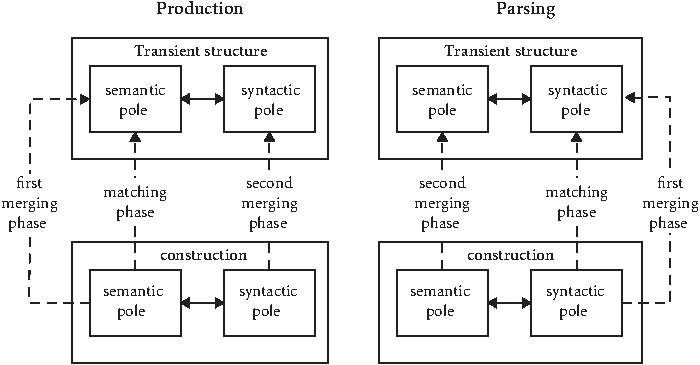
\includegraphics[width=.98\textwidth]{Figures/production-parsing-fcg.pdf}
\caption{\label{fig-matching-merging-trijp}Generation and parsing in FCG \citep[\page 99]{vanTrijp2013a}}
\end{figure}%

\subsubsection{Argument Structure Constructions}

Fluid Construction Grammar assumes a phrasal approach to argument structure, that is, it is assumed that lexical items enter
into phrasal configurations that contribute independent meaning \citep{vanTrijp2011a}. The FCG
approach is one version of implementing Goldberg's plugging approach to argument structure
constructions \citep{Goldberg95a}. Van Trijp suggests that every lexical item comes with a representation of
potential argument roles like Agent, Patient, Recipient, and Goal. Phrasal argument structure
constructions are combined with the respective lexical items and realize a subset of the argument
roles, that is they assign them to grammatical functions. Figure~\vref{fig-as-trijp} shows an
example: the verb \emph{sent} has the semantic roles Agent, Patient, Recipient, and Goal  (upper left
of the figure). Depending
on the argument structure construction that is chosen, a subset of these roles is selected for
realization.\footnote{%
  It is interesting to note here that \citet[\page 141]{vanTrijp2011a} actually suggests a lexical
  account since every lexical item is connected to various phrasal constructions via coapplication
  links. So every such pair of a lexical item and a phrasal construction corresponds to a lexical
  item in Lexicalized Tree Adjoining Grammar (LTAG). See also \citew[\page 25]{MWArgSt} on
  Goldberg's assumption that every lexical item is associated with phrasal constructions.

Note that such coapplication links are needed since without them the approach cannot account for
cases in which two or more argument roles can only be realized together but not in isolation or in
any other combination with other listed roles.
}
%\todostefan{Are there Agent Goal verbs or Patient Recipient or Patient Goal verbs that allow for
%  patterns that are impossible for sent?}
The figures show the relation between sender, sent, and sendee and more the more abstract semantic
roles and the relation between these roles and grammatical functions for the sentences in (\mex{1}):
\eal
\ex He sent her the letter.
\ex He sent the letter.
\ex The letter was sent to her.
\zl
While in (\mex{0}a) the agent, the patient and the recipient are mapped to grammatical functions,
only the agent and the patient are mapped to grammatical functions in (\mex{0}b). The recipient is
left out. (\mex{0}c) shows an argument realization in which the sendee is realized as a \emph{to}
  phrase. According to van Trijp this semantic role is not a recipient but a goal. 


\begin{figure}
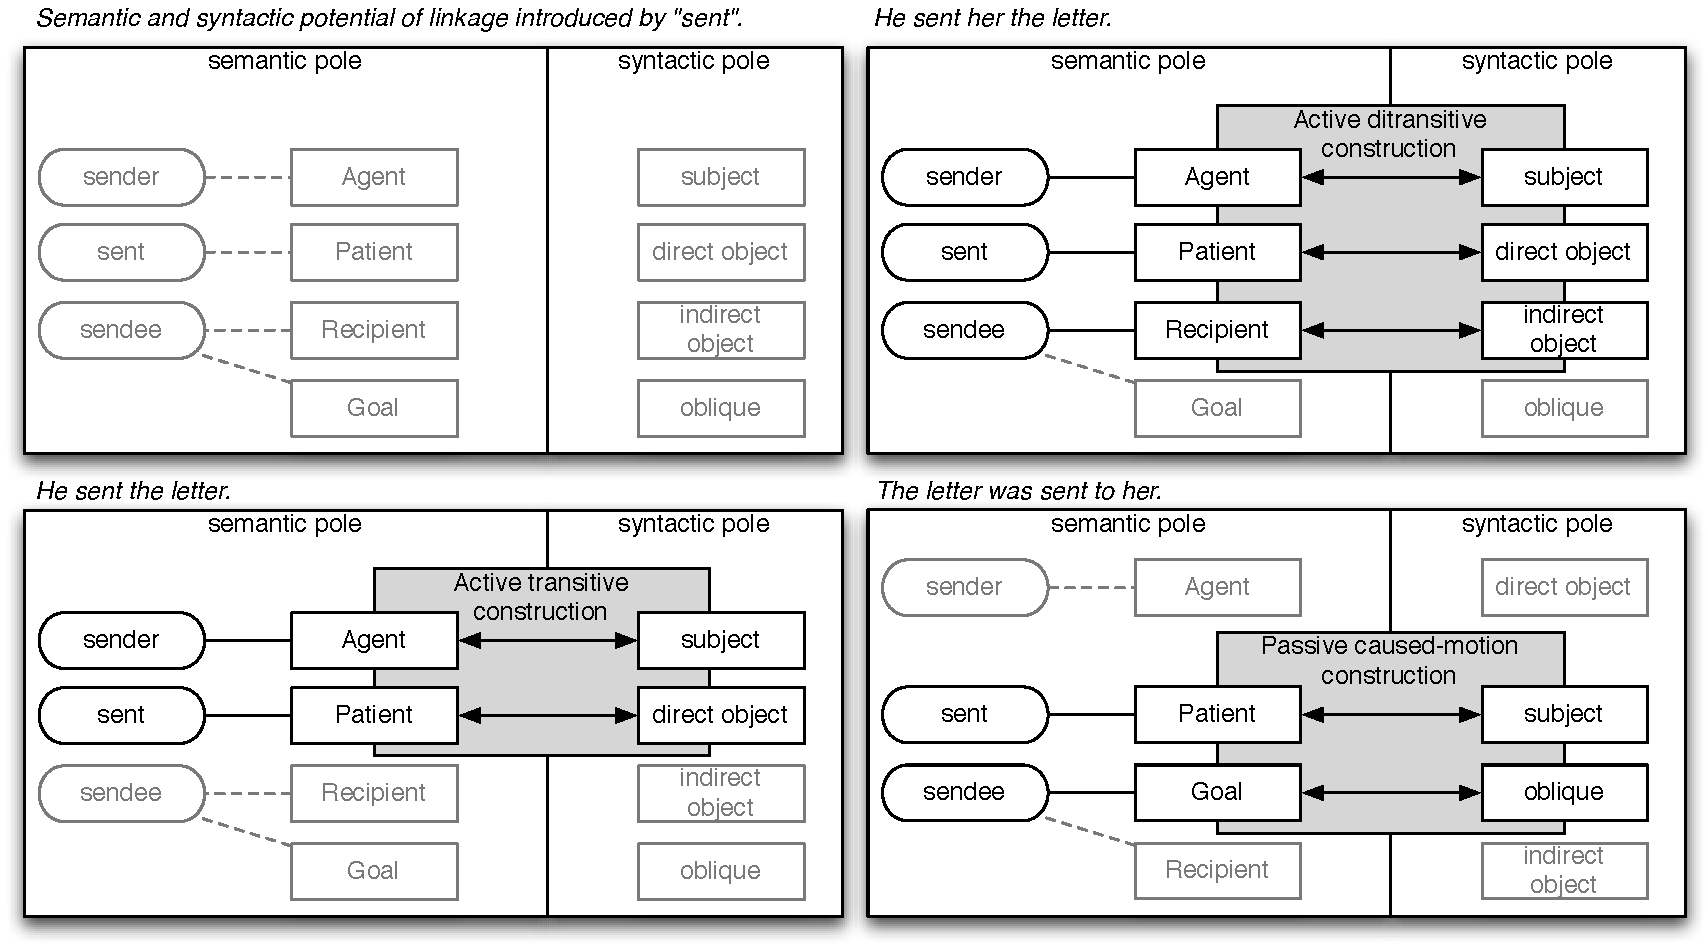
\includegraphics[width=\textwidth]{Figures/2011-van-Trijp.pdf}
\caption{\label{fig-as-trijp}Lexical items and phrasal constructions. Figure %taken 
from \citew[\page 122]{vanTrijp2011a}}
\end{figure}%

Note that under such an approach, it is necessary to have a passive variant of every active
construction. For languages that allow for the combination of passive and impersonal constructions,
one would be forced to assume a transitive-passive-impersonal construction. As was argued in
\citew[Section~2.6]{Mueller2006d} free datives (commodi/incommodi) in German can be added to almost
any construction. They interact with the dative passive and hence should be treated as
arguments. So, for the resultative construction one would need an active variant, a passive variant,
a variant with dative argument, a variant with dative argument and dative passive, and a middle variant.
While it is technically possible to list all these patterns and it is imaginable that we store all
this information in our brains, the question is whether such listings really reflect our linguistic
knowledge. If a new construction comes into existence, lets say an active sentence pattern with a
nominative and two datives in German, wouldn't we expect that this pattern can be used in the
passive? While proposals that establish relations between active and passive constructions would
predict this, alternative proposals that just list the attested possibilities do not.

\addlines[2]
The issue of how such generalizations should be captured was discussed in connection with the
organization of the lexicon in HPSG \citep{Flickinger87,Meurers2001a}. In the lexical world, one could simply categorize all verbs according to their
valence and say that \emph{loves} is a transitive verb and the passive variant \emph{loved} is an
intransitive verb. Similarly \emph{gives} would be categorized as a ditransitive verb and
\emph{given} as a two-place verb. Obviously this misses the point that \emph{loved} and \emph{given}
share something: they both are related to their active form in a systematic way. This kind of
generalization is captured by lexical rules that relate two lexical items. The respective
generalizations that are captured by lexical rules are called a horizontal generalizations as compared to vertical generalizations, which
describe relations between subtypes and supertypes in an inheritance hierarchy.

The issue is independent of the lexical organization of knowledge, it can be applied to phrasal
representations as well. Phrasal constructions can be organized in hierarchies (vertical), but the
relation between certain variants is not covered by this. The analog to the lexical rules in a
lexical approach are GPSG-like metarules in a phrasal approach. So what seems to be missing in FCG
is something that relates phrasal patterns, \eg allostructions (\citealp{Cappelle2006a}; \citealp[\page
  116]{Goldberg2014a}, see also footnote~\ref{fn-allostructions}).


\subsubsection{Fusion, matching and merging}

As was pointed out by \citet[\page 89--90]{Dowty89b-u}, checking for semantic compatibility is not sufficient
when deciding whether a verb may enter (or be fused with) a certain construction. The example is
the contrast between \emph{dine}, \emph{eat}, and \emph{devour}. While the thing that is eaten may
not be realized with \emph{dine}, its realization is optional with \emph{eat} and obligatory with
\emph{devour}. So the lexical items have to come with some information about
this. 

\Citet{vanTrijp2011a} and \citet{SvT2011a} make an interesting suggestion that could help
here: every verb comes with a list of potential roles and argument structure constructions can pick
subsets of these roles (see Figure~\ref{fig-as-trijp}). This is called \emph{matching}: introducing new argument roles is not allowed. 
This would make it possible to account for \emph{dine}: one could
say that there is something that is eaten, but that no Theme role is made available for linking to
the grammatical functions. This would be a misuse of thematic roles for syntactic purposes though
since \emph{dine} is semantically a two-place predicate. To account for the extension of argument roles as it is observed in the
Caused"=Motion Construction\is{construction!Caused"=Motion} \citep[Chapter~7]{Goldberg95a}, \citet{SvT2011a} suggest a process called \emph{merging}. Merging is seen
as a repair strategy: if an utterance involves an intransitive verb and some other material, the
utterance cannot be processed with matching alone. For example, when processing Goldberg's example
in (\mex{1}), \emph{he sneezed} could be parsed, but \emph{the foam} and \emph{off the cappuccino}
would be unintegrated (see Chapter~\ref{chap-phrasal} for an extended discussion of such constructions).
\ea
He sneezed the foam off the cappuccino.\footnote{%
\citew[\page 42]{Goldberg2006a}.
}
\z
So, \citet[\page 319--320]{SvT2011a} suggest that only if regular constructions cannot apply, merging is
allowed. The problem with this is that human language is highly ambiguous and in the case
at hand this could result in situations in which there is a reading for an utterance, so that the
repair strategy would never kick in. Consider (\mex{1}):\footnote{%
  I apologize for these examples \ldots. An English example that shows that there may be ambiguity
  between the depictive and the resultative construction is the following one that is due to
  \citet{Haider2016b}:
  \ea
  They cooked the chicken dry.
  \z
  I use the German example below since the resultative reading is strongly preferred over the
  depictive one.
}
\ea
\label{ex-schlag-den-mann-tot}
\gll Schlag den Mann tot!\\
     beat   the man  dead\\
\glt `Beat the man to death!' or `Beat the dead man!'
\z
(\mex{0}) has two readings: the resultative reading in which \emph{tot} `dead' expresses the result of the
beating and another reading in which \emph{tot} is a depictive predicate. The second reading is
dispreferred, since the activity of beating dead people is uncommon, but the structure is parallel to
other sentences with depictive predicates:
\ea
\gll Iss den Fisch roh!\\
     eat the fish raw\\
\z
The depictive reading can be forced by coordinating \emph{tot} with a predicate that is not a
plausible result predicate:
\ea
\gll Schlag ihn tot oder lebendig!\\
     beat   him dead or alive\\
\glt `Beat him when he is dead or while he is alive!'
\z
So, the problem is that (\ref{ex-schlag-den-mann-tot}) has a reading which does not require the invocation of the repair mechanism: \emph{schlug} `beat' is used with the transitive
construction and \emph{tot} is an adjunct (see \citealp{Winkler97a}). However, the more likely analysis of (\ref{ex-schlag-den-mann-tot}) is the one
with the resultative analysis, in which the valence frame is extended by an oblique element. So this
means that one has to allow the application of merging independent of other analyses that might be possible.
As \citet[\page 320]{SvT2011a} note, if merging is allowed to apply freely, utterances like
(\mex{1}a) will be allowed and of course (\mex{1}b) as well.
\eal
\ex[*]{
She sneezed her boyfriend.
}
\ex[*]{
She dined a steak.
}
\zl
In (\mex{0}) \emph{sneeze} and \emph{dined} are used in the transitive construction.

The way out of this dilemma is to establish information in lexical items that specifies in which
syntactic environments a verb can be used. This information can be weighted and for instance the
probability of \emph{dine} to be used transitively would be extremely low. Steels and van Trijp
would connect their lexical items to phrasal constructions via so-called coapplication links and the
strength of the respective link would be very low for \emph{dine} and the transitive construction and
reasonably high for \emph{sneeze} and the Caused"=Motion Construction\is{construction!Caused"=Motion}. This would explain the
phenomena (and in a usage"=based way), but it would be a lexical approach, as it is common in CG, HPSG,
SBCG, and DG.

\subsubsection{Long-distance dependencies}
\label{sec-fcg-nld}

%\addlines
\Citet{vanTrijp2014a} compares the \slasch-based approaches that are used in GPSG, HPSG, and SBCG
with the approach that he suggests within the framework of FCG. He claims that there are fundamental
differences between SBCG and FCG and assigns SBCG to the class of generative grammars, while
placing FCG in the class of cognitive"=functional approaches. He claims that his
cognitive"=functional approach is superior in terms of completeness, explanatory adequacy, and
theoretical parsimony (p.\,2). What \citet{vanTrijp2014a} suggests is basically an analysis that was
suggested by \citet{Reape2000a} in unpublished work (see \citew{Reape94a} for a published version of
an linearization"=based approach and \citew{Kathol2000a,Babel,Mueller99a,Mueller2002b} for
linearization"=based approaches that despite of being linearization"=based assume the \slasch approach for nonlocal dependencies). Van Trijp
develops a model of grammar that allows for discontinuous constituents and just treats the
serialization of the object in sentences like (\mex{1}) as an alternative linearization option.
\eal
\ex This book, I read.
\ex What did the boy hit?
\zl
Van Trijp's analysis involves several units that do not normally exist in phrase structure grammars,
but can be modeled via adjacency constraints or which represent relations between items which are part
of lexical representations in HPSG/SBCG anyway. An example is the subject-verb anchor that connects
the subject and the verb to represent the fact that these two items play an important functional
role. Figure~\vref{fig-what-did-the-boy-hit} shows the analysis of (\mex{1}).
\ea
What did the boy hit?
\z
\begin{figure}
\begin{forest}
for tree={l sep+=5mm}
%l sep+=10mm
[TRANSITVE-CLAUSE-UNIT, name=tcu
  [NP-UNIT-1, name=np1
    [PRO [what]] ]
  [AUX,tier=det, no edge, name=aux [did] ]
  [NP-UNIT-2, name=np2
    [DET, tier=det [the]]
    [N   [boy]] ]
  [VP-UNIT, name=vp
    [V [hit] ] ]
]
\draw (vp.south)--(aux.north);
\node (topic) [base left=of tcu]
    {
        TOPIC-UNIT
    };
\draw[dashed] (topic.south)--(np1.north);
\node (focus) [below=0mm of tcu.south west]
    {
        FOCUS-UNIT
    };
\draw[dashed] (focus.south)--(np1.north);
\draw[dashed] (focus.south)--(aux.north);
\node (sau) [base right= of tcu]
    {
        SV-ANCHOR-UNIT
    };
\draw[dashed] (sau.south)--(vp.north);
\draw[dashed] (sau.south)--(np2.north);
\end{forest}
\caption{\label{fig-what-did-the-boy-hit}The analysis of \emph{What did the boy hit?} according to
  \citet[\page 265]{vanTrijp2014a}}
\end{figure}%
As can be seen in the figure, van Trijp also refers to information structural\is{information structure} terms
like topic and focus. It should be noted here that the analysis of information structure has quite
some history in the framework of HPSG  \citep{EV96a, 
Kuhn95b,Kuhn96a, 
GuntherMaienborn1999,
Wilcock2001a,Wilcock2005a, 
deKuthy2002a,Paggio2005a-u, 
%\citet{Webelhuth2007a-u}, 
Bildhauer2008a,BC2010a}. The fact that information structure is not talked about in syntax
papers like \citew{Sag2012a} does not entail that information structure is ignored or should be
ignored in theories like HPSG and SBCG. So much for completeness. The same holds of course for
explanatory adequacy. This leaves us with theoretical parsimony, but before I comment on this, I
want to discuss van Trijp's analysis in a little bit more detail in order to show that many of his claims
are empirically problematic and that his theory therefore cannot be explanatory since empirical
correctness is a precondition for explanatory adequacy.

Van Trijp claims that sentences with nonlocal dependency constructions in English start with a
topic.\footnote{%
\Citet[\page 256]{vanTrijp2014a} uses the following definitions for topic and focus: ``Topicality is defined in terms of aboutness: the topic of an utterance
is what the utterance is `about'. Focality is defined in terms of salience:
focus is used for highlighting the most important information given the
current communicative setting.''
} Bresnan's sentences in (\ref{bsp-fronted-focus}) and (\ref{bsp-fronted-topic}) were discussed on page~\pageref{bsp-fronted-focus}
\citep[\page 97]{Bresnan2001a} and are repeated below for convenience:
\ea
\label{bsp-fronted-focus-two}
Q: What did you name your cat?\\
A: Rosie I named her. (\emph{Rosie} = \textsc{focus})
\z
\ea
\label{bsp-fronted-topic-two}
Q: What did you name your pets?\\
A: My dog, I named Harold. My cat, I named Rosie. (\emph{my dog}, \emph{my cat} = \textsc{topic})
\z
These sentences show that the pre-subject position is not unambiguously a topic or a focus
position. So, a statement saying that the fronted element is a topic is empirically not correct. If this position is to be associated with an information structural function, this
association has to be a disjunction admitting both topics and focused constituents.

A further problematic aspect of van Trijp's analysis is that he assumes that the auxiliary \emph{do}
is an object marker (p.\,10, 22) or a non-subject marker (p.\,23). It is true that \emph{do} support is not necessary in subject questions like
(\mex{1}a), but only in (\mex{1}b), but this does not imply that all items that are followed by
\emph{do} are objects.
\eal
\ex Who saw the man?
\ex Who did John see?
\zl
\addlines
First, \emph{do} can be used to emphasize the verb:
\ea
Who \emph{did} see the man?
\z
Second, all types of other grammatical functions can precede the verb:
\eal
\settowidth\jamwidth{(prepositional object)}
\ex Where did you see the man? \jambox{(adverbial)}
\ex How tall is the man? \jambox{(predicative)}
\ex What did John consider Peter? \jambox{(predicative)}
\ex What does this book cost? \jambox{(adverbial)}
\ex About what did you talk? \jambox{(prepositional object)}
\zl
And finally, even a subject can appear in front of \emph{do} if it is extracted from another clause:
\ea
\settowidth\jamwidth{(prepositional object)}
Who does he think saw this man? \jambox{(subject)}
\z
%
% Auch die linke Peripherie kann man ja einfach als kontinuierlich einordnen. Brauche Beleg für
% Extraposition aus pränominalem Adjunkt. Das würde mögliche Diskontinuität zeigen.
%
%% Van Trijp does not address the issue of island constraints. Extraction islands are areas that nobody
%% can leave, that is, extraction is excluded. For instance, it is impossible to extract from the
%% prenominal area in English and German (Ross' Left Branch Condition).
%\ea
%der die Frau liebende Mann, die ... erfunden hat
%%  and it is also impossible to
%% extract out of a relative clause:
%% % Er könnte sagen, dass Relativsätze immer kontinuierlich sein müssen.
%% \ea
%% This man$_i$, I saw a women [who likes \_$_i$ ].
%% \z
%% \slasch"=based models assume that relative clauses involve internal nonlocal dependencies, but no
%% \slasch dependency leaves the relative clause. This is ensured by the schemata that combine the
%% relative pronoun and the remaining clause.

There is a further empirical problem: approaches that assume that a filler is related to its origin
can explain scope ambiguities that only arise when an element is extracted. Compare for instance the
sentence in (\mex{1}a) with the sentences in (\mex{1}b, c): although the order of \emph{oft} `often' and
\emph{nicht} `not' in (\mex{1}a) and (\mex{1}c) is the same, (\mex{1}a) is ambiguous but (\mex{1}c) is
not.
\eal
\ex 
\gll Oft liest er das Buch nicht.\\
     often reads he the book not\\
\glt `It is often that he does not read the book.' or `It is not the case that he reads the book
often.'
\ex
\gll dass er das Buch nicht oft liest\\
     that he the book not often reads\\
\glt `that it is not the case that he reads the book often'
\ex
\gll dass er das Buch oft nicht liest\\
     that he the book often not reads\\
\glt `that it is often that he does not read the book'
\zl
(\mex{0}a) has the two readings that correspond to (\mex{0}b) and (\mex{0}c). A purely
linearization"=based approach probably has difficulties to explain this. A \slasch"=based approach
can assume that (\mex{0}a) has a gap (or some similar means for the introduction of nonlocal
dependencies) at the position of \emph{oft} in (\mex{0}b) or (\mex{0}c). The gap information is
taken into account in the semantic composition at the site of the gap. This automatically accounts
for the observed readings.

Another empirical problem that has to be solved is the existence of extraction path
marking\is{extraction path marking}
languages. \citet*{BMS2001a} list a number of languages in which elements vary depending on the
existence or absence of a gap in a constituent they attach to. For instance, Irish has
complementizers that have one form if the clause they attach to has an element extracted and another
form if it does not. \slasch-based proposals can account for this in a straight-forward way: the
fact that a constituent is missing in a phrase is represented in the \slashv of the trace and this
information is percolated up the tree. So even complex structures contain the information that there
is a constituent missing inside them. Complementizers that are combined with sentences therefore can
select sentences with \slashvs that correspond to the form of the complementizer.
Van Trijp's answer to this challenge is that all languages are different
\citep[\page 263]{vanTrijp2014a} and that the evidence from one language does not necessarily mean that the analysis for that language is
also appropriate for another language. While I agree with this view in principle (see
Section~\ref{sec-syntactic-universals}), I do think that extraction is a rather fundamental property
of languages and that nonlocal dependencies should be analyzed in parallel for those languages that
have it.


\subsection{Coordination}
\label{sec-coordination}

One of the success stories of non-transformational grammar is the \slasch-based analysis of nonlocal dependencies
by \citet{Gazdar81}. This analysis made it possible for the first time to explain Ross's Across the Board
Extraction\is{Across the Board Extraction} \citep{Ross67}. The examples were already discussed on
page~\pageref{ex-atb-gazdar} and are repeated here for convenience:
\eal\settowidth\jamwidth{(= S/NP \& S/NP)}
\label{ex-atb-gazdar-two}
\ex[]{ The kennel     which Mary made and Fido sleeps in has been stolen.	 \jambox{(= S/NP \& S/NP)}
}
\ex[]{ The kennel in which Mary keeps drugs and Fido sleeps has been stolen.	\jambox{(= S/PP \& S/PP)}
}
\ex[*]{The kennel (in) which Mary made and Fido sleeps has been stolen.     \jambox{(= S/NP \& S/PP)}
}
\zl
The generalization is that two (or more) constituents can be coordinated if they have identical
syntactic categories and identical \slashvs. This explains why \emph{which} and \emph{in which} in
(\mex{0}a,b) can fill two positions in the respective clauses. Now, theories that do not use a
\slashf for the percolation of information about missing elements have to find different ways to
make sure that all argument slots are filled and that the correct correspondence between extracted
elements and the respective argument role is established. Note that this is not straightforward in
models like the one suggested by van Trijp, since he has to allow the preposition \emph{in} to be
combined with some material to the left of it that is simultaneously also the object of
\emph{made}. Usually an NP cannot simply be used by two different heads as their argument. As an
example consider (\mex{1}a):
\eal
\ex[*]{
John said about the cheese that I like.
}
\ex[]{
John said about the cheese that I like it.
}
\zl
If it would be possible to use material several times, a structure for (\mex{0}a) would be possible
in which \emph{the cheese} is the object of the preposition \emph{about} and of the verb
\emph{like}. This sentence, however, is totally out: the pronoun \emph{it} has to be used to fill
the object slot.


\subsection{Discontinuous constituents and performance models}

Van Trijp points out that SBCG does not have a performance model and contrasts this with FCG. On
page~252 he states:
\begin{quote}
So parsing starts by segmenting the utterance
into discrete forms, which are then categorized into words by morphological
and lexical constructions, and which can then be grouped together as
phrases (see Steels, 2011b, for a detailed account of lexico-phrasal
processing in FCG). So the parser will find similar constituents for all
four utterances, as shown in examples (21--24). Since auxiliary-\emph{do} in
example (24) falls outside the immediate domain of the VP, it is not yet
recognized as a member of the VP.

All of these phrases are disconnected, which means that the grammar
still has to identify the relations between the phrases. \citep[\page 252]{vanTrijp2014a}
\end{quote}
In his (21)--(24), van Trijp provides several tree fragments that contain NPs for subject and object and states that
these have to be combined in order to analyze the sentences he discusses. This is empirically
inadequate: if FCG does not make the competence/performance distinction, then the way utterances are
analyzed should reflect the way humans process language (and this is what is usually claimed about FCG). However, all we know about human language
processing points towards an incremental processing, that is, we process information as soon as it
is available. We start to process the first word taking into account all of the relevant aspects
(phonology, stress, part of speech, semantics, information structure) and come up with an hypothesis
about how the utterance could proceed. As soon as we have two
words processed (in fact even earlier: integration already happens during the processing of words) we integrate the second word
into what we know already and continue to follow our hypothesis, or revise it, or simply fail. See
Section~\ref{Abschnitt-Inkrementelle-Verarbeitung} for details on processing and the discussion of
experiments that show that processing is incremental. So, we have to say that van Trijp's analysis
fails on empirical grounds: his modeling of performance aspects is not adequate.

The parsing scheme that van Trijp describes is pretty much similar to those of computational HPSG parsers, but
these usually come without any claims about human performance. Modeling human performance is rather complex
since a lot of factors play a role. It is therefore reasonable to separate competence and
performance and continue to work the way it is done in HPSG and FCG. This does not mean that
performance aspects should not be modeled, in fact psycholinguistic models using HPSG have been
developed in the past \citep{Konieczny96a-u}, but developing both a grammar with large coverage and
the performance model that combines with it demands a lot of resources.

\subsection{Discontinuity vs.\ Subject-Head and Head-Filler Schema}
\label{sec-discontinuous-constituents-fcg}

I now turn to parsimony: van Trijp uses a subject-verb anchor construction that combines the subject
and the main verb. Because of examples like (\mex{1}) it must be possible to have discontinuous subject-verb constructions:\footnote{%
  Unless modals and tense auxiliaries are treated as main verbs (which they should not in English), constructions with
  modals seem to be another case where the subject and the main verb are not adjacent:
  \eal
  \ex Peter will read the book.
  \ex Peter has read the book.
  \zllast
} 
\ea
Peter often reads books.
\z
\largerpage
But if such constructions can be discontinuous one has to make sure that (\mex{1}b) cannot be an
instantiation of the subject-verb construction:
\eal
\ex[]{
The boy I think left.
}
\ex[*]{
I the boy think left.
}
\zl
Here it is required to have some adjacency between the subject and the verb it belongs to, modulo
some intervening adverbials. This is modelled quite nicely in phrase structure grammars that have a
VP node. Whatever the internal structure of such a VP node may be, it has to be adjacent to the
subject in sentences like  (\mex{-1}) and (\mex{0}a) above. The dislocated element has to be adjacent to the complex
consisting of subject and VP. This is what the Filler-Head Schema does in HPSG and SBCG. Van Trijp
criticizes SBCG for having to stipulate such a schema, but I cannot see how his grammar can be
complete without a statement that ensures the right order of elements in sentences with fronted
elements.

Van Trijp stated that FCG differs from what he calls generative approaches in that it does not want
to characterize only the well-formed utterances of a language. According to him, the parsing direction
 is much more liberal in accepting input than other theories. So it could well be that he
is happy to find a structure for (\mex{0}b). Note though that this is incompatible with other claims
made by van Trijp: he argued that FCG is superior to other theories in that it comes with a performance
model (or rather in not separating competence from performance at all). But then (\mex{0}b) should be
rejected both on competence and performance grounds. It is just unacceptable and speakers reject it
for whatever reasons. Any sufficiently worked out theory of language has to account for this.


\subsection{Restricting discontinuity}
\label{sec-restricting-discont}

There is a further problem related to discontinuity. If one does not restrict continuity, then
constituent orders like (\mex{1}b) are admitted by the grammar:
\eal
\ex[]{
\gll Deshalb klärt, dass Peter kommt, ob Klaus spielt.\\
     therefore resolves that Peter comes whether Klaus plays\\
\glt `Therefore that Peter comes resolves whether Klaus will play.'
}
\ex[*]{
\gll Deshalb klärt dass ob Peter Klaus kommt spielt.\\
     therefore resolves that whether Peter Klaus comes plays\\
}
\zl
The interesting thing about the word salad in (\mex{0}b) is that the constituent order within the
\emph{dass} clause and within the \emph{ob} clause is correct. That is, the complementizer precedes
the subject, which in turn precedes the verb. The problem is that the constituents of the two
clauses are mixed. 
%% Note that the clausal arguments can appear in both orders:
%% \ea
%% \gll Deshalb klärt, ob Klaus spielt, dass Peter kommt.\\
%%      therefore resolves whether Klaus comes that Peter comes\\
%% \z
%% Therefore 

In a model that permits discontinuous constituents, one cannot require that all parts of an argument have
to be arranged after all parts that belong to another argument since discontinuity is used to
account for nonlocal dependencies. So, it must be possible to have \emph{Klaus} before other
arguments (or parts of other arguments) since \emph{Klaus} can be extracted. An example of mixing
parts of phrases is given in (\mex{1}):
\ea
\gll Dieses Buch hat der Mann mir versprochen, seiner Frau zu geben, der gestern hier aufgetreten ist.\\
     this   book has the man  me  promised     his    wife to give   who yesterday here performed is\\
\glt `The man who performed here yesterday promised me to give this book to his wife.'
\z 
%\addlines[2]
We see that material that refers to \emph{der Mann} `the man', namely the relative clause \emph{der gestern
  hier aufgetreten ist} `who performed here yesterday', appears to the right. And the object of
\emph{geben} `to give', which would normally
be part of the phrase \emph{dieses Buch seiner Frau zu geben} `this book his wife to give' appears to the left. So, in general it
is possible to mix parts of phrases, but this is possible in a very restricted way only. Some
dependencies extend all the way to the left of certain units (fronting) and others all the way to the right
(extraposition). Extraposition is clause-bound, while extraction is not. In approaches like GPSG,
HPSG and SBCG, the facts are covered by assuming that constituents for a complete clause are
continuous apart from constituents that are fronted or extraposed. The fronted and extraposed
constituents are represented in \slasch and \extra (\citealp{Keller95b};
\citealp[Section~13.2]{Mueller99a}; \citealp{Crysmann2013a}), respectively, rather than in valence features,
so that it is possible to require of constituents that have all their valents saturated to be
continuous \citep[\page 294]{Mueller99g}.

Summing up the discussion of parsimony, it has to be said that van Trijp has to provide the details
on how continuity is ensured. The formalization of this is not trivial and only after this is done
can FCG be compared with the \slasch"=based approach.

In addition to all the points discussed so far, there is a logical flaw in van Trijp's argumentation.
He states that:
\begin{quote}
whereas the filler-gap analysis cannot explain \textsc{why} \emph{do}-support does not occur
  in \emph{wh}-questions where the subject is assigned questioning focus, this follows naturally
from the interaction of different linguistic perspectives in this paper's
approach. \citep[\page 263]{vanTrijp2014a}
\end{quote}
The issue here is whether a filler-gap analysis or an analysis with discontinuous
constituents is suited better for explaining the data. A correct argumentation against the filler-gap analysis would require a proof that information structural or other functional constraints
cannot be combined with this analysis. This proof was not provided and in fact I think it cannot be
provided since there are approaches that integrate information structure. Simply pointing out that a
theory is incomplete does not falsify a theory. This point was already made in my review of
\citew{Boas2003a} and in a reply to \citet{Boas2014a}. See \citew[655--656]{Mueller2005a},
\citew[Chapter~20]{MuellerLehrbuch1}, and \citew[Footnote~15]{MWArgStReply}.

The conclusion about the FCG analysis of nonlocal dependencies is that there are some empirical
flaws that can be easily fixed or assumptions that can simply be dropped (role of \emph{do} as object marker, claim that
the initial position in English fronting construction is the topic), some empirical shortcomings
(coordination, admittance of illformed utterances with discontinuous constituents), some empirical
problems when the analysis is extended to other languages (scope of adjuncts in German), and the
parsimony of the analyses is not really comparable since the restrictions on continuity are not
really worked out (or at least not published). If the formalization of restrictions on continuity in FCG turns out to be even
half as complex as the formalization that is necessary for accounts of nonlocal dependencies
(extraction and extraposition) in linearization"=based HPSG that \citet{Reape2000a}
suggested,\footnote{%
  See \citew{KP95a} for a linearization"=based account of extraposition. This account is
  implemented in the Babel System \citep{Babel}. See \citep{Mueller99g} on restricting
  discontinuity. Linearization"=based approaches were argued to not be able to account for
  apparent multiple frontings in German \citep{Mueller2005d,MuellerGS} and hence
  linearization"=based approaches were replaced by more traditional variants that allow for
  continuous constituents only.
} the \slasch"=based analysis would be favorable.

In any case, I do not see how nonlocal dependencies could be used to drive a wedge between SBCG and
FCG. If there are functional considerations that have to be taken into account, they should be
modeled in both frameworks. In general, FCG should be more restrictive than SBCG since FCG claims to
integrate a performance model, so both competence and performance constraints should be operative. I
will come back to the competence/""performance distinction in the following section, which is a more
general comparison of SBCG and FCG.

\subsubsection{Comparison to Sign-Based Construction Grammar/HPSG}


According\indexhpsgstart\indexsbcgstart to \citet{vanTrijp2013a}, there are the differences shown in Table~\vref{table-differences-SBCG-FCG}.
%% \begin{itemize}
%% \item
%% \label{fcg-sbcg-generative} SBCG embraces a generative conception of linguistic theory, whereas FCG adopts a
%%   cognitive-functional approach (p.\,89)
%% \item
%% \end{itemize}
%
% moved to top
These differences will be discussed in the following subsections.
\begin{table}
\caption{\label{table-differences-SBCG-FCG}Differences between SBCG and FCG according to \citet[\page 112]{vanTrijp2013a}}
\begin{tabular}{@{}lll@{}}\hline\hline
Scientific model    & Theoretical physics           & Evolutionary theory\\
                    & (abstract calculus)           &  (complex adaptive system)\\
Linguistic approach & Generative                    & Cognitive-functional\\
                    & (competence model)            & (parsing and production)\\
Formalization       & Mathematical                  & Computational\\ 
                    & (amenable for implementation) & (implemented)\\
Constructions       & Static type constraints       & Dynamic mappings\\
Constructicon       & Signature and grammar         & Open-ended inventory\\
Processing          & Assumption of processing-     & Bidirectional processing\\
                    & independence                  & model\\\hline\hline
\end{tabular}
\end{table}%

\subsubsubsection{Competence/performance distinction}
\label{sec-performance-cxg}

As\is{competence|(}\is{performance|(} for the linguistic approach, the use of the term \emph{generative} is
confusing. What van Trijp means -- and also explains in the paper -- is the idea that one should
separate competence and performance. We will deal with both the generative-enumerative
vs.\ constraint-based view and with the competence/performance distinction in more detail in the
Chapters~\ref{Abschnitt-Generativ-Modelltheoretisch} and~\ref{Abschnitt-Diskussion-Performanz},
respectively. Concerning the cognitive-functional approach, van Trijp writes:
\begin{quote}
The goal of a cognitive-functional grammar, on the other hand, is to explain
how speakers express their conceptualizations of the world through language
(= \emph{production}) and how listeners analyze utterances into meanings (= \emph{parsing}).
Cognitive-functional grammars therefore implement both a competence and a
processing model. \citep[\page 90]{vanTrijp2013a}
\end{quote}
\largerpage
It is true that HPSG and SBCG make a competence/performance distinction \citep{SW2011a}. HPSG
theories are theories about the structure of utterances that are motivated by distributional
evidence. These theories do not contain any hypothesis regarding brain activation, planning of
utterances, processing of utterances (garden path effects) and similar things. In fact, none of the
theories that are discussed in this book contains an explicit theory that explains all these
things. I think that it is perfectly legitimate to work in this way: it is legitimate to study the
structure of words without studying their semantics and pragmatics, it is legitimate to study
phonology without caring about syntax, it is legitimate to deal with specific semantic problems
without caring about phonology and so on, provided there are ways to integrate the results of such
research into a bigger picture. In comparison, it is wrong to develop models like those developed in current
versions of Minimalism\indexmp (called Biolinguistics\is{Biolinguistics}), where it is assumed that utterances are derived in
phases\is{phase} (NPs, CPs, depending on the variant of the theory) and then shipped to the interfaces\is{interface} (spell
out and semantic interpretation). This is not what humans do (see
Chapter~\ref{Abschnitt-Diskussion-Performanz}).\footnote{%
Attempts to integrate current Minimalist theories with psycholinguistic findings \citep{Phillips2003a} are
incompatible with core principles of Minimalism like the \emph{No Tampering Condition}\is{No
  Tampering Condition (NTC)} of \citet{Chomsky2008a}.
}
But if we are neutral with respect towards such
issues, we are fine. In fact, there is psycholinguistic work that couples HPSG grammars to
performance models \citep{Konieczny96a-u} and similar work exists for TAG \citep{SJ93a,DK2008a-u}. 

%\addlines[-1]
Finally, there is also work in Construction Grammar that abstracts away from performance
considerations. For instance, Adele Goldberg's book from \citeyear{Goldberg95a} does
not contain a worked out theory of performance facts. It contains boxes in which grammatical
functions are related to semantic roles. So this basically is a competence theory as well. Of course
there are statements about how this is connected to psycholinguistic findings, but this is also true
for theories like HPSG, SBCG and Simpler Syntax \citep[\page 600]{Jackendoff2011a} that explicitly make the competence/performance distinction.\is{competence|)}\is{performance|)}

\subsubsubsection{Mathematical formalization vs.\ implementation}

The difference between mathematical and computational formalization is a rather strange distinction to make. I
think that a formal and precise description is a prerequisite for implementation (see the discussion
in Section~\ref{sec-formalization-gb} and Section~\ref{sec-formalization-minimalism}). Apart from this, a computer implementation of SBCG is
trivial, given the systems that we have for processing HPSG grammars. In order to show this, I want
to address one issue that van Trijp discusses. He claims that SBCG cannot be directly
implemented. On issues of complexity of constraint solving systems he quotes \citep[Section~4.2.2]{LM2006a}:
\begin{quote}
Actual implementations of HPSG typically handle the problem by guiding the linguistic processor
using a (rule-based) phrase structure backbone, but the disadvantage of this approach is that the ``organization and formulation of the grammar is different from
that of the linguistic theory'' \citep[Section~4.2.2]{LM2006a}. \citep[\page 108]{vanTrijp2013a}
\end{quote}
\largerpage
He concludes:
\begin{quote}
Applying all these observations to the operationalization of SBCG, we can
conclude that an SBCG grammar is certainly amenable for computational implementation because of its formal explicitness. There are at least two computational
platforms available, mostly used for implementing HPSG-based grammars, whose
basic tenets are compatible with the foundations of SBCG: LKB \citep{Copestake2002a}
and TRALE\is{TRALE} (Richter 2006). However, none of these platforms supports a `direct'
implementation of an SBCG grammar as a general constraint system, so SBCG's
performance-independence hypothesis remains conjecture until proven otherwise.
\end{quote}
%\addlines
There are two issues that should be kept apart here: efficiency and faithfulness to the
theory. First, as Levine and Meurers point out, there were many constraint solving systems at the
beginning of the 90's. So there are computer systems that can and have been used to implement
and process HPSG grammars. This is very valuable since they can be used for direct verification of
specific theoretical proposals. As was discussed by Levine and Meurers, trying to solve constraints
without any guidance is not the most efficient way to deal with the parsing/generation
problem. Therefore, additional control-structure was added. This control structure is used for
instance in a parser to determine the syntactic structure of a phrase and other constraints will
apply as soon as there is sufficient information available for them to apply. For instance, the
assignment of structural case happens once the arguments of a head are realized. Now, is it bad to
have a phrase structure backbone? One can write down phrase structure grammars that use phrase
structure rules that have nothing to do with what HPSG grammars usually do. The systems TRALE \citep*{MPR2002a-u,Penn2004a-u} and
LKB will process them. But one is not forced to do this. For instance, the grammars that I developed
for the CoreGram project \citep{MuellerCoreGramBrief,MuellerCoreGram} are very close to the linguistic theory. To see that this is really the
case, let us look at the Head-Argument Schema. The Head-Argument Schema is basically the type
\type{head-argument-phrase} with certain type constraints that are partly inherited from its
supertypes. The type with all the constraints was given on page~\pageref{head-arg-schema-hfp} and is
repeated here as (\mex{1}):
\largerpage[2]
\eas
\label{head-arg-schema-hfp-zwei}
(syntactic) constraints on \type{head-complement-phrase}:\\
\onems[head-complement-phrase~]{
synsem$|$loc$|$cat  \ms{ head   & \ibox{1} \\
                          comps & \ibox{2}
                        }\\
head-dtr$|$synsem$|$loc$|$cat \ms{ head   & \ibox{1} \\
                                   comps & \ibox{2} $\oplus$ \sliste{ \ibox{3} }
                                 } \\
non-head-dtrs   \sliste{ [ synsem \ibox{3} ] }
}
\zs
%\addlines
This can be translated into phrase structure grammar rules in a straight-forward way:
\eal
\ex \onems[head-complement-phrase~]{
synsem$|$loc$|$cat  \ms{ head   & \ibox{1} \\
                          comps & \ibox{2}
                        }\\
head-dtr \ibox{4} $|$synsem$|$loc$|$cat \ms{ head   & \ibox{1} \\
                                   comps & \ibox{2} $\oplus$ \sliste{ \ibox{3} }
                                 } \\
non-head-dtrs   \sliste{ \ibox{5} [ synsem \ibox{3} ] }
} $\to$ \ibox{4}, \ibox{5}
\ex \onems[head-complement-phrase~]{
synsem$|$loc$|$cat  \ms{ head   & \ibox{1} \\
                          comps & \ibox{2}
                        }\\
head-dtr \ibox{4} $|$synsem$|$loc$|$cat \ms{ head   & \ibox{1} \\
                                   comps & \ibox{2} $\oplus$ \sliste{ \ibox{3} }
                                 } \\
non-head-dtrs   \sliste{ \ibox{5} [ synsem \ibox{3} ] }
} $\to$ \ibox{5}, \ibox{4}
\zl
The left hand side of the rule is the mother node of the tree, that is, the sign that is licensed by
the schema provided that the daughters are present. The right hand side in (\mex{0}a) consists of
the head daughter \iboxt{4} followed by the non-head daughter \ibox{5}. We have the opposite order
in (\mex{0}b), that is, the head daughter follows the non-head daughter. The two orders correspond
to the two orders that are permitted by LP-rules: the head precedes its argument if it is marked
\textsc{initial}+ and it follows it if it is marked \textsc{initial}$-$.

The following code shows how (\mex{0}b) is implemented in TRALE:
\begin{verbatim}
arg_h rule (head_complement_phrase,
          synsem:loc:cat:head:initial:minus,
          head_dtr:HeadDtr,
          non_head_dtrs:[NonHeadDtr]
         )
  ===>
cat> NonHeadDtr,
cat> HeadDtr.
\end{verbatim}
A rule starts with an identifier that is needed for technical reasons like displaying intermediate
structures in the parsing process in debugging tools. A description of the mother node follows and
after the arrow we find a list of daughters, each introduced by the operator \verb+cat>+.\footnote{%
  Other operators are possible in TRALE. For instance, \texttt{sem\_head} can be used to guide the
  generator. This is control information that has nothing to do with linguistic theory and not
  necessarily with the way humans process natural language. There is also a \texttt{cats} operator,
  which precedes lists of daughters. This can be used to implement phrase structures with more than
  one non-head daughter.%
}
Structure sharing is indicated by values with capital letters. The above TRALE rule is a
computer"=readable variant of (\mex{0}b) additionally including the explicit specification of the value of {\initial}.  

Now, the translation of a parallel schema using a \textsc{mother} feature like (\mex{1}a) into a phrase structure rule is almost as simple:
\eal
\ex \onems[head-complement-cx~]{
mother$|$synsem$|$loc$|$cat  \ms{ head   & \ibox{1} \\
                                  comps & \ibox{2}
                        }\\
head-dtr$|$synsem$|$loc$|$cat \ms{ head   & \ibox{1} \\
                                   comps & \ibox{2} $\oplus$ \sliste{ \ibox{3} }
                                 } \\
non-head-dtrs   \sliste{ [ synsem \ibox{3} ] }
}

\ex 
\ibox{6} $\to$ \ibox{4}, \ibox{5} where \onems[head-complement-cx~]{
mother \ibox{6} $|$synsem$|$loc$|$cat  \ms{ head   & \ibox{1} \\
                          comps & \ibox{2}
                        }\\
head-dtr \ibox{4} $|$synsem$|$loc$|$cat \ms{ head   & \ibox{1} \\
                                             comps & \ibox{2} $\oplus$ \sliste{ \ibox{3} }
                                 } \\
non-head-dtrs   \sliste{ \ibox{5} [ synsem \ibox{3} ] }
}
\zl
(\mex{0}b) is only one of the two phrase structure rules that correspond to (\mex{0}a), but since
the other one only differs from (\mex{0}b) in the ordering of \iboxt{4} and \iboxt{5}, it is not
given here.

For grammars in which the order of the elements corresponds to the observable order of the
daughters in a \textsc{dtrs} list, the connection to phrase structure rules is even simpler:
\ea 
\ibox{1} $\to$ \ibox{2} where \ms[construction~]{
mother & \ibox{1} \\
dtrs   & \ibox{2}
}
\z
%\addlines[2]
The value of \textsc{dtrs} is a list and hence \iboxt{2} stands for the list of daughters on the right
hand side of the phrase structure rule as well. The type \type{construction} is a supertype of all
constructions and hence (\mex{0}) can be used to analyze all phrases that are licensed by the
grammar. In fact, (\mex{0}) is one way to put the meta constraint in (\ref{meta-construction-statemnet}).

So, this shows that the version of SBCG that has been developed by \citet{Sag2012a} has a
straightforward implementation in TRALE.\footnote{%
A toy fragment of English using a \textsc{mother} feature and phrase structure rules with specifications
of the kind given above can be downloaded at \url{https://hpsg.hu-berlin.de/Fragments/SBCG-TRALE/}.%
}
The question remains whether ``SBCG's performance"=independence hypothesis remains conjecture until proven otherwise'' as van Trijp sees
it. The answer is: it is not a conjecture since any of the old constraint-solving systems of the
nineties could be used to process SBCG. The question of whether this is efficient is an engineering
problem that is entirely irrelevant for theoretical linguistics. Theoretical linguistics is
concerned with human languages and how they are processed by humans. So whether some processing system
that does not make any claims about human language processing is efficient or not is absolutely
irrelevant. Phrase structure-based backbones are therefore irrelevant as well, provided they refer
to the grammar as described in theoretical work.  

\largerpage
\enlargethispage{6pt}
Now, this begs the question whether there is a contradiction in my claims. On
page~\pageref{page-sbcg-formalization} I pointed out that SBCG is lacking a formalization in
Richter's framework \citep{Richter2004a-u}. Richter and also \citet{LM2006a} pointed out that there are problems with
certain theoretically possible expressions and it is these expressions that mathematical linguists care
about. So the goal is to be sure that any HPSG grammar has a meaning and that it is clear what it
is. Therefore, this goal is much more foundational than writing a single grammar for a particular fragment
of a language. There is no such foundational work for FCG since FCG is a specific toolkit that has been used
to implement a set of grammars.

\subsubsubsection{Static constraints vs.\ dynamic mappings and signature $+$ grammar vs.\ open-endedness}

%\addlines
On very interesting feature of Fluid Construction Grammar is its fluidity, that is there are certain
constraints that can be adapted if there is pressure, the inventory of the theory is open-ended, so
categories and features can be added if need be.

Again, this is not a fundamental difference between HPSG/SBCG and FCG. An HPSG grammar fragment of a
specific language is a declarative representation of linguistic knowledge and as such it of course
just represents a certain fragment and does not contain any information how this set of constraints
evolved or how it is acquired by speakers. For this we need specific theories about language
evolution/"language change/"language acquisition. This is parallel to what was said about the
competence/performance distinction, in order to account for language evolution we would have to have
several HPSG grammars and say something about how one developed from the other. This will involve
weighted constraints, it will involve recategorization of linguistic items and lots more.\footnote{%
  There are systems that use weighted constraints. We had a simple version of this in the
  German HPSG grammar that was developed in \verbmobil project \citep{MK2000a} already. Further
  theoretical approaches to integrate weighted constraints are \citew{Brew95a} and more recently
  \citew{Guzman-Naranjo2015a}. Usually such weighted constraints are not part of theoretical papers,
  but there are exceptions as for instance the paper by Briscoe and Copestake about lexical rules \citep{BC99a}.
} So basically HPSG has to be extended, has to be paired with a model about
language evolution in the very same way as FCG is.



\subsubsubsection{Theoretical physics vs.\ Darwinian evolutionary theory}

\largerpage[2]
Van Trijp compares SBCG and FCG and claims that SBCG follows the model of theoretical physics --
like Chomsky does --, while FCG adopts a Darwinian model of science -- like Croft does --, the difference
being that SBCG makes certain assumptions that are true of all languages, while FCG does not make
any a priori assumptions. The fundamental assumptions made in both theories are that the
objects that we model are best described by feature value pairs (a triviality). FCG assumes that
there is always a syntactic and a semantic pole (fundamental assumption in the system) and
researchers working in HPSG/SBCG assume that if languages have certain phenomena, they will be
analyzed in similar ways. For instance, if a language has nonlocal dependencies, these will be
analyzed via the \slasch mechanism. However, this does not entail that one believes that grammars of
all languages have a \slashf. And in fact, there may even be languages that do not have valence
features \citep{KM2010a-u}, which may be a problem for FCG since it relies on the SYN-pole for the
matching phase. So as far as SBCG is concerned, there is considerable freedom to choose features
that are relevant in an analysis, and of course additional features and types can be assumed in case
a language is found that provides evidence for this. The only example of a constraint provided by van Trijp that is possibly too strong
 is the locality constraint imposed by the \textsc{mother}
feature. The idea about this feature is that everything that is of relevance in a more nonlocal
context has to be passed up explicitly. This is done for nonlocal dependencies (via \slasch) and for instance also
for information concerning the form of a preposition inside of a PP (via \textsc{pform} or more
recently via \form). Certain verbs require prepositional objects and restrict
the form of the preposition. For instance, \emph{wait} has to make sure that its prepositional
object has the preposition \emph{for} in it. Since this information is usually available only at the
preposition, it has to be passed up to the PP level in order to be directly selectable by the
governing verb. 
\ea
I am waiting for my man.
\z 
%\addlines[2]
So, assuming strict locality of selection requires that all phenomena that cannot be treated locally
have to be analyzed by passing information up.
%% \footnote{%
%%   It should also be noted that \citet[\page 111]{vanTrijp2013a} draws hasty conclusions when he
%%   writes: \emph{the locality of SBCG constructions, which entails that all languages can best be
%% described as constraints on local trees.} Depending on the definition of tree 
%% }
Assuming strict locality is a design decision that does not have any empirical consequences, as far
as it does not rule out any language or construction in principle. It just requires that information
has to be passed up that needs to be accessed at higher nodes. As I have shown in Section~\ref{sec-SbCxG},
the locality constraint is easily circumvented even within SBCG and it makes the analysis of idioms
unnecessarily complicated and unintuitive, so I suggest dropping the \textsc{mother} feature. But even if \textsc{mother} is kept, it is not justified to draw a
distinction between SBCG and FCG along the lines suggested by van Trijp. 

Independent of the \textsc{mother} issue, the work done in the CoreGram project
\citep{MuellerCoreGramBrief,MuellerCoreGram} shows that one can derive generalizations in a
bottom-up fashion rather than imposing constraints on grammars in a top-down way. The latter paper
discusses Croft's methodological considerations and shows how methodological pitfalls are
circumvented in the project. HPSG/SBCG research differs from work in Chomskyan frameworks in not
trying to show that all languages are like English or Romance or German or whatever, rather
languages are treated on their own as it is common in the Construction Grammar community. This does
not imply that there is no interest in generalizations and universals or near universals or tendencies, but again
the style of working and the rhetoric in HPSG/SBCG is usually different from the ones in Mainstream
Generative Grammar. Therefore, I think that the purported difference
between SBCG and FCG does not exist.

\subsubsubsection{Permissiveness of the theories}

\largerpage[2]
Van Trijp claims that HPSG/SBCG is a ``generative grammar'' since its aim is to account for and admit only
grammatical sentences. FCG on the other hand is more permissive and tries to get the most out of the
input even if it is fragmentary or ungrammatical (see also \citealp[\page 166]{Steels2013a}). While it is an engineering decision to be able to parse ungrammatical input --  and 
 there are most certainly systems for the robust processing of HPSG grammars \citep*{KKN2000a-u,Copestake2007a-u}, it is also
clear that humans cannot parse everything. There are strong constraints whose violations cause measurable
effects in the brain. This is something that a model of language (that includes competence and
performance factors or does not make the difference at all) has to explain. The question is
what the cause of deviance is: is it processing complexity? Is it a category mismatch? A clash in
information structure? So, if FCG
permits structures that are not accepted by human native speakers and that do not make any sense
whatsoever, additional constraints have to be added. If they are not added, the respective FCG
theory is not an adequate theory of the language under consideration. Again, there is no difference
between HPSG/SBCG and FCG.  

\subsubsubsection{A note on engineering}

%\addlines[2]
A problematic property of work done in FCG is that linguistic and engineering aspects are mixed.\footnote{%
This is not a problem if all FCG papers are read as papers documenting the FCG-system (see
Footnote~\ref{Steels-FCG-System} on page~\pageref{Steels-FCG-System}) since then it
would be necessary to include these technical details. If the FCG papers are to be read as
theoretical linguistics papers that document a certain Construction Grammar analysis, the Lisp statements
and the implementational details are simply an obstacle.
} Certain bookkeeping features that are needed only
for technical reasons appear in linguistic papers, technical assumptions that are made to get a
parser running are mixed with linguistic constraints. Bit vector\is{bit vector} encodings that are used to
represent case information are part of papers about interesting case systems. There is certainly
nothing wrong with bit vector encodings. They are used in HPSG implementations as well
(\citealp[\page 55]{Reape91}; \citealp[\page 269]{Babel}), but this is
not mixed into the theoretical papers. 

It was a big breakthrough in the 80's when theoretical linguists and computational linguists started
working together and developed declarative formalisms that were independent of specific parsers and
processing systems. This made it possible to take over insights from a lot of linguists who were not
concerned with the actual implementation but took care of finding linguistic generalizations and
specifying constraints. Since this separation is given up in FCG, it will remain an engineering
project without much appeal to the general linguist.%
\indexhpsgend\indexsbcgend



\section{Summary and classification}

\largerpage
\begin{sloppypar}
There are currently three formalized variants of Construction Grammar: Sign"=Based Construction
Grammar, Embodied Construction Grammar, and Fluid Construction Grammar. The first two variants can
be viewed as notational variants of (Constructional) HPSG\indexhpsg (for SBCG with regard to this
point, see \citew[\page 411]{Sag2007a} and \citew[\page 486]{Sag2010b}), or put differently, sister
theories of HPSG. This is also true to a large extend for FCG, although \citet{vanTrijp2013a} spends
25 pages working out the alleged differences. As I have shown in Section~\ref{sec-fcg}, HPSG and FCG are
rather similar and I would say that these theories are sister theories as well. 
\end{sloppypar}

Due to the origins of all three theories, respective analyses can differ quite considerably: HPSG is a strongly lexicalized theory, where
phrasal dominance schemata have only been increasingly more used in the last ten years under the
influence of Ivan Sag\ia{Ivan A. Sag}. The phrasal dominance schemata that Ivan Sag uses in
his work are basically refinements of schemata that were present in earlier versions of
HPSG. Crucially, all phenomena that interact with valence receive a lexical analysis \citep*[Section~2.3]{SBK2012a}.
In CxG, on the other hand, predominantly phrasal analyses are adopted due to the influence of Adele Goldberg\ia{Adele E.\ Goldberg}.%

As already emphasized in Chapter~\ref{Kapitel-HPSG}, these are only tendencies that do not apply to all researchers working in the
theories in question.



\section*{Exercises}

\begin{enumerate}
\item Find three examples of utterances whose meaning cannot be derived from the meaning of the individual words. Consider how
one could analyze these examples in Categorial Grammar (yes, Categorial Grammar).
\end{enumerate}

\section*{Further reading}

There are two volumes on Construction Grammar in German: \citew{FS2006a-ed-not-crossreferenced} and \citew{SF2008a-ed}.
\citet{Deppermann2006a} discusses Construction Grammar from the point of view of conversational
analysis.  The 37(3) volume of the \textit{Zeitschrift für germanistische Linguistik} from 2009 was
also devoted to Construction Grammar.  \citew{Goldberg2003b} and \citew{Michaelis2006a} are overview
articles in English. Goldberg's books constitute important contributions to Construction Grammar
\citeyearpar{Goldberg95a,Goldberg2006a,Goldberg2009a}.  \citet{Goldberg95a} has argued against
lexical analyses such as those common in GB, LFG, CG, HPSG, and DG. These arguments can be
invalidated, however, as will be shown in Section~\ref{sec-lr-phrasal-psycho}.
\citet{Sag97a}, \citet{Borsley2006a}, \citet{Jacobs2008a} and \citet{ML2009a} give examples of
constructions that require a phrasal analysis if one wishes to avoid postulating empty elements.
\citet{Jackendoff2008a} discusses the noun"=preposition"=noun construction that can only be properly
analyzed as a phrasal construction (see Section~\ref{Abschnitt-Phrasale-Konstruktionen}). The
discussion on whether argument structure constructions should be analyzed phrasally or lexically
\citep{Goldberg95a,Goldberg2006a,Mueller2006d} culminated in a series of papers
\citep{Goldberg2013a} and a target article by \citet{MWArgSt} with several responses in the same
volume.

Tomasello's publications on language acquisition
\citep{Tomasello2000a,Tomasello2003a,Tomasello2005a,Tomasello2006a}\nocite{Tomasello95a} constitute
a Construction Grammar alternative to the Principle \& Parameters theory of acquisition as it does
not have many of the problems that P\&P analyses have (for more on language acquisition, see
Chapter~\ref{chap-acquisition}).  For more on language acquisition and Construction Grammar,
see \citew{Behrens2009a}.

\citet{Dabrowska2004a} looks at psycholinguistic constraints for possible grammatical theories.\is{Construction Grammar (CxG)|)}  

%      <!-- Local IspellDict: en_US-w_accents -->



% vanTrijp2014:7 FCG no locality of selection
% He seems to refer to discontinuity her, but this is independent
